%------------------------------------------------------------------------------
%
% システムプログラミング教科書
%
%------------------------------------------------------------------------------
\documentclass[a4paper,11pt,twocolumn]{ltjsbook}      % lualatex の場合
\usepackage{mySty}
%------------------------------------------------------------------------------
% はじまり
\begin{document}
\frontmatter
%------------------------------------------------------------------------------
% 表紙
\title{システムプログラミング\\Ver. 0.0.0}
\author{徳山工業高等専門学校\\情報電子工学科}
\date{}
\maketitle

%------------------------------------------------------------------------------
% 著作権表示
\thispagestyle{empty}
\onecolumn
~
\vfill
\begin{flushleft}
Copyright \copyright ~~ 2017 - 2019 by \\
Dept. of Computer Science and Electronic Engineering, \\
Tokuyama College of Technology, JAPAN
\end{flushleft}

\vspace{0.8cm}
本ドキュメントはCC-BY-SA 4.0 ライセンスによって許諾されています。

本ドキュメントは
CC-BY-SA 3.0 de ライセンス,
CC-BY-SA 4.0 ライセンス
で許諾された著作物を含みます.

(CC-BY-SA 3.0 de ライセンス全文は
\url{https://creativecommons.org/licenses/by-sa/3.0/de/}で,
CC-BY-SA 4.0 ライセンス全文は
\url{https://creativecommons.org/licenses/by-sa/4.0/deed.ja}で確認できます.)

%------------------------------------------------------------------------------
% 目次
\setcounter{tocdepth}{2}
\tableofcontents

% 本文
%\twocolumn
\mainmatter

\part{OSの機能を使用してみよう}
\chapter{システムプログラミング}

本講義は,
オペレーティングシステム本体が持つ機能を直接に使用するような
システムプログラムの作成を行う.
システムプログラムをプログラミングする経験の中から,
オペレーティングシステム本体が備えている機能の役割りや必要性を体感的に学ぶ.

\section{システムプログラムとは}
システムプログラムは,
乱暴な言い方をするとアプリケーション以外のプログラムのことである.
\figref{systemConstruct}にコンピュータシステムの構成を簡単に示す.
この図でアプリケーションプログラムとハードウェアを除いた,
オペレーティングシステム本体(カーネル),
ライブラリ,ミドルウェア,ユーティリティ,プログラム開発環境は
システムプログラムである.

\begin{myfig}{btp}{コンピュータシステムの構成}{systemConstruct}
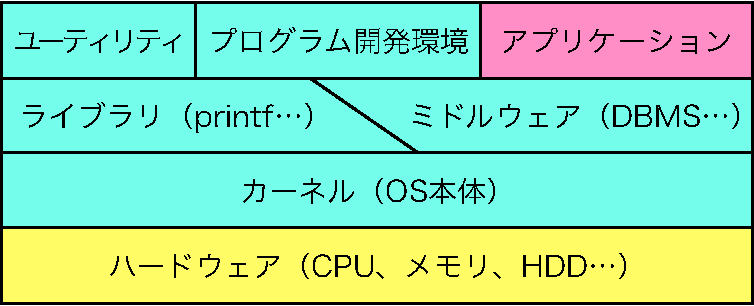
\includegraphics[scale=0.8]{Fig/systemConstruct-crop.pdf}
\end{myfig}

\begin{enumerate}
\item カーネル(OSの本体)
\item ライブラリ(プログラムが使用するサブルーチン,DLL ...)
\item ミドルウェア(DBMS,Webサーバ ...)
\item ユーティリティ(ファイル操作,時計,シェル,システム管理 ...)
\item プログラム開発環境
(エディタ,コンパイラ,アセンブラ,リンカ,インタプリタ ...)
\end{enumerate}

\section{システムプログラミングとは}
システムプログラムを作成することをシステムプログラミングと呼ぶ.
本講義では,
システムプログラムの中でもユーティリティの作成を行う.
WindowsやmacOSではGUIを備えた様々なユーティリティが準備されている\footnote{
WindowsやmacOSの場合でも,
GUIを備えていないユーティリティも,多数,存在する.}.
しかし,本講義の目的は
「システムプログラミングを通してのオペレーティングシステムの体感的な理解」
であるので,GUIの作成にエネルギーを費やしたくはない.
そこで,CLI(Command Line Interface)のユーティリティを作成する.

本講義では,
オペレーティングシステムを体感的に理解するために,
オペレーティングシステムの機能を直接に使用する
\emph{簡単なCLI版のユーティリティプログラムの作成(プログラミング)}を行う.

\section{システムコール}
一つのコンピュータシステムの中で複数のプログラムが同時に作動していることは,
誰もが体験的に知っていると思う.
しかし,それらのプログラムが勝手にシステムの\emph{資源}にアクセスすると,
資源の管理が正しく行えない可能性があり具合が悪い.
例えばハードディスクでは,
複数のプログラムが勝手にファイルを作成すると,
複数のファイルがハードディスクの同じ領域に割当てられるかも知れない.

そこで,
資源にアクセスするのはオペレーティングシステムの
本体である\emph{カーネル}だけに限り,
カーネルが代表して資源を管理することにする.
他のプログラムはカーネルに依頼し目的を達成する.
その様子を図を使って説明する.

\begin{myfig}{btp}{システムコールなし}{noSystemcall}
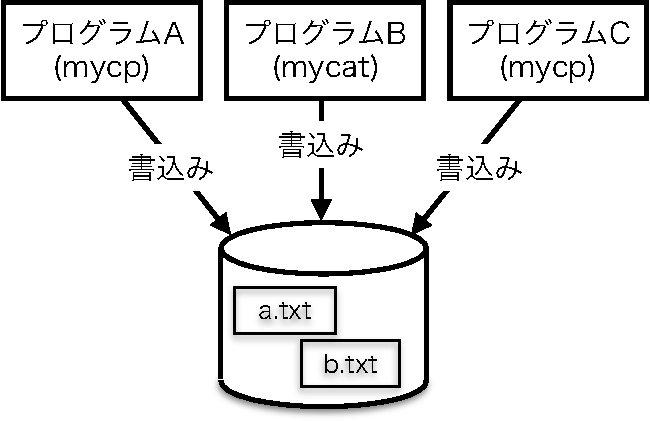
\includegraphics[scale=0.8]{Fig/noSystemcall-crop.pdf}
\end{myfig}

\begin{myfig}{btp}{システムコールあり}{systemcall}
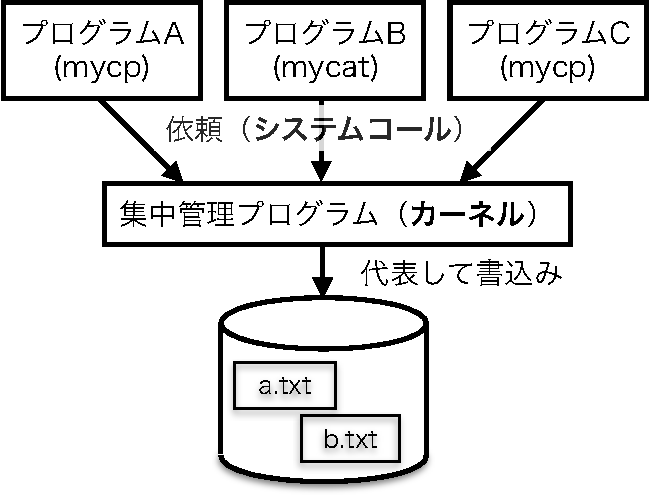
\includegraphics[scale=0.8]{Fig/systemcall-crop.pdf}
\end{myfig}

\begin{enumerate}
\item \figref{noSystemcall}のように,
システムの中で同時に複数のプログラムが実行され,
それぞれが\emph{資源}にアクセスする必要がある.
図の例では,
三つのプログラムが同時にハードディスクにファイルを作ろうとしている.
複数のプログラムが勝手にハードウェア
\emph{資源}(ハードディスク,プリンタ,メモリ ...)を操作すると具合が悪い.
\item そこで,\figref{systemcall}のように資源を集中管理するプログラム,
\emph{カーネル}(OSの本体)を導入する.
一般のプログラムは\emph{システムコール}を用いてカーネルに処理を依頼する.
\end{enumerate}

\section{システムコールの使用}
C言語から,
UNIX(macOS)のシステムコールを直接に利用することが可能である.
以下の章では,
macOS上でC言語を用いてシステムコールを直接に使用するプログラムを作成しながら,
システムコールの機能を確認する.
また,ユーティリティプログラムの簡単版を作成する.

\begin{quote}
\begin{lstlisting}[language=C++, numbers=none]
// ディレクトリを作るユーティリティプログラム(mymkdir)の例
...
int main(int argc, char *argv[]) {
  if (argc!=2) {
    // エラー処理
    ...
  }
  mkdir(argv[1]);    // ディレクトリを作るシステムコール
  return 0;
}
\end{lstlisting}
\end{quote}

\section*{練習問題}
\begin{enumerate}
%\renewcommand{\labelenumi}{\ttfamily \arabic{chapter}.\arabic{enumi}}
% \setlength{\leftskip}{1em}

\item ハードウェア\emph{資源}の例を挙げなさい.

\item \emph{カーネル}の役割りを本章の範囲で説明しなさい.

\item \emph{システムコール}の役割りを簡単に説明しなさい.

\item 自分がいつも使用しているコンピュータやスマートフォンの
オペレーティングシステムの種類(Windows?)を調べなさい.
\end{enumerate}

 % システムプログラム
\chapter{ファイル入出力システムコール}

この章ではファイルの読み書きを行うシステムコールを紹介し,
これらを直接に使用したユーティリティプログラムを作成してみる.
C言語を用いると,
システムコールと同じ名前の関数を呼び出すことで
システムコールを呼び出すことができる.
例えばopenシステムコールを使用するときは,
\|open()|関数を呼び出す.

\section{高水準入出力と低水準入出力}
C言語の入門で勉強した
\|fopen()|,
\|printf()|,
\|puts()|,
\|putchar()|,
\|fprintf()|,
\|fputs()|,
\|fputc()|,
\|scanf()|,
\|getchar()|,
\|fgets()|,
\|fgetc()|,
\|fclose()|...
等は\emph{高水準入出力}関数と呼ばれる.
これに対してシステムコールを直接使用する入出力を\emph{低水準入出力}と呼ぶ.

\tabref{hilevelVsSystemcall}に対応を示すように,
高水準入出力関数は内部でファイル入出力を行うシステムコールを呼び出している.
つまり,種類や機能が豊富な高水準入出力は,
数種類の基本的な機能しか提供しない低水準入出力を用いて
実現されていることになる.


\begin{mytable}{btp}{高水準入出力関数とシステムコール}{hilevelVsSystemcall}
\begin{tabular}{l | l}\hline\hline
\emph{高水準入出力関数} & \emph{対応するシステムコール} \\\hline
\texttt{fopen()}      & open システムコール \\
\texttt{printf()}     & write システムコール \\
\texttt{putchar()}    & write システムコール \\
%\texttt{fputs()}      & write システムコール \\
\texttt{fputc()}      & write システムコール \\
...          & ...                     \\
\texttt{scanf()}      & read システムコール \\
\texttt{getchar()}    & read システムコール \\
%\texttt{fgets()}      & read システムコール \\
\texttt{fgetc()}      & read システムコール \\
...          & ...                      \\
\texttt{fclose()}     & close システムコール \\
\end{tabular}
\end{mytable}

\section{openシステムコール}
ファイルのオープンに使用するシステムコールである.
詳細なマニュアルは UNIX(macOS) のターミナルで,
\texttt{man 2 open}と入力すると表示される\footnote{
\texttt{man}はUNIXマニュアルを表示するユーティリティプログラムである.
引数の\texttt{2}が表す第2章は,「システムコール」を解説している.
本文中の例は「UNIXマニュアルの第2章の\texttt{open}」の項目を表示する.}.

\begin{description}
\item[書式1](オープンするだけの場合)

\begin{lstlisting}[numbers=none]
#include <fcntl.h>
int open(const char *path, int oflag);
\end{lstlisting}

\item[解説]
openシステムコールを使用するプログラムの先頭では,
\|fcntl.h|をインクルードする必要がある.
openシステムコールは
正常時には\emph{ファイルディスクリプタ}(ゼロ以上の整数)を返す
\footnote{stdinのファイルディスクリプタが0,
stdoutのものが1,stderrのものが2なので3以降の番号を返す.}.
エラーが発生した時は\|-1|を返す.
エラー原因は\|perror()|関数で表示できる.

\item[引数]
\|path|はオープンまたは作成するファイルのパス(名前),
\|oflag|はオープンの方法を表す。
\|oflag|は\tabref{open}の記号定数を\texttt{|}\footnote{
\texttt{|}は,C言語のビット毎の論理和演算子である.}で接続して書く.
表の左側の記号定数を一つと,
右側の記号定数を幾つか組合せることができる.
例えばファイルの内容を消してから書き込み用にオープンしたい場合は,
\verb;O_WRONLY|O_TRUNC;のように書く.

\begin{mytable}{btp}{openシステムコールの第2引数\texttt{oflag}}{open}
\begin{tabular}{l | c | l}
\hline\hline
\emph{以下の一つ} & と & \emph{以下のいくつか} \\\hline
\|O_RDONLY|(読み出し用) &    & \|O_APPEND|(追記)  \\
\|O_WRONLY|(書き込み用) & +  & \|O_CREAT|(作成)   \\
\|O_RDWR|(読み書き両用) &    & \|O_TRUNC|(切詰め) \\
                      &    & ...      \\
\end{tabular}
\end{mytable}

\item[使用例](書式1)

\begin{lstlisting}[numbers=none]
#include <fcntl.h>
...
int fdr, fdw, fda;
fdr=open("r.txt", O_RDONLY);              // 読み出し用にオープン
fdw=open("w.txt", O_WRONLY);              // 書き込み用にオープン
fda=open("a.txt", O_WRONLY|O_APPEND);     // 追記用にオープン

if (fdw<0) {                              // エラーチェック
  perror("w.txt");                        //  原因の表示
  exit(1);                                //  エラー終了
}
\end{lstlisting}


\begin{figure}[tb]
\begin{framed}
\subsection*{ファイルの保護モード}
open システムコールの第3引数(\|mode|)は次のような 12bit の値である.

\begin{center}
{\ttfamily\small\begin{tabular}{|c|c|c||c|c|c||c|c|c||c|c|c|}
\multicolumn{1}{c}{11} &
\multicolumn{1}{c}{10} &
\multicolumn{1}{c}{ 9} &
\multicolumn{1}{c}{ 8} &
\multicolumn{1}{c}{ 7} &
\multicolumn{1}{c}{ 6} &
\multicolumn{1}{c}{ 5} &
\multicolumn{1}{c}{ 4} &
\multicolumn{1}{c}{ 3} &
\multicolumn{1}{c}{ 2} &
\multicolumn{1}{c}{ 1} &
\multicolumn{1}{c}{ 0} \\\hline
s  & s  & t & r & w & x & r & w & x & r & w & x \\\hline
\multicolumn{3}{c}{省略} &
\multicolumn{3}{c}{ユーザ} &
\multicolumn{3}{c}{グループ} &
\multicolumn{3}{c}{その他} 
\end{tabular}}
\end{center}

最初の 3bit の意味は難しいのでここでは説明を省略する.
他のビットは \|rwx| のどれかである.
\|rwx| の意味は次の通りである.

\begin{tabular}{c c l}
\texttt{r} & : & \emph{r}ead 可(読み出し可能)   \\
\texttt{w} & : & \emph{w}rite 可(書き込み可能)   \\
\texttt{x} & : & e\emph{x}ecute 可(実行可能)
\end{tabular}

例えば,第8ビットが \|1| だったら、
ユーザ(ファイルの所有者)が read (読み出し)可能の意味になる.
%逆に \|0|なら read 不可の意味になる.
ファイルのモードやユーザ(所有者),グループは次のようにして確認できる.

\begin{lstlisting}[numbers=none]
$ ls -l a.txt
-rw-r--r--  1 sigemura  staff  0 Apr 11 05:53 a.txt
$
\end{lstlisting}

a.txt ファイルのモードの下位9ビットが \|110100100| である.
所有者は sigemura,
グループは staff である.
このファイルは sigemura が読み書きができる.
staff グループに属するユーザは読むことだけできる.
その他のユーザも読むことだけできる.
\end{framed}
\end{figure}

\item[書式2](ファイル作成もする場合)

\|oflag|に\|O_CREAT|を含む場合は,
該当ファイルが存在しないなら新規作成してからオープンする.
新規作成するファイルの\emph{保護モード}を\|mode|で指定する.

\begin{lstlisting}[numbers=none]
#include <fcntl.h>
int open(const char *path, int oflag, mode_t mode);
\end{lstlisting}

\|mode_t| は,16bit の整数型(16bit \|int|)である.
\|mode| は,作成されるファイルの保護モードである.
\|mode| は,8進数で記述することが多い\footnote{
C言語では,数値を \texttt{0} で書き始めると8進数の意味になる.}.
8進数と保護モードの対応は次のようになる.

{\ttfamily\begin{center}\begin{tabular}{l l}
0: --- ~~~ & 4: r-- \\
1: --x     & 5: r-x \\
2: -w-     & 6: rw- \\
3: -wx     & 7: rwx
\end{tabular}\end{center}}

\item[使用例](書式2)

\begin{lstlisting}[numbers=none]
fd=open("a.txt", O_WRONLY|O_CREAT, 0644);  // 作るファイルのモードは rw-r--r-- になる
\end{lstlisting}

\end{description}

\section{readシステムコール}
読み出し用にオープン済みのファイルからデータを読み出すシステムコールである.
1回目はファイルの先頭から指定されたバイト数を読み出す.
2回目以降は,ファイルの前回読み終わった位置から続きを読み出す.
このようにファイルの先頭から順に読み書きする方式は,
\emph{シーケンシャルアクセス(順次アクセス)}と呼ばれる.
後で紹介するwriteシステムコールもシーケンシャルアクセスを行う.

\begin{description}
\item[書式](詳しくは\texttt{man 2 read}で調べる.)

\begin{lstlisting}[numbers=none]
#include <unistd.h>
ssize_t read(int fildes, void *buf, size_t nbyte);
\end{lstlisting}

\item[解説]
read システムコールを使用するプログラムの先頭では,
\|unistd.h|をインクルードする必要がある.
オープン済みのファイルディスクリプタを渡し,
ファイルからデータを読み出す.

read システムコールは\|ssize_t|型(64bit \|int|型)の値を返す.
値は正常時には読んだデータのバイト数(正の値),
EOF では \|0| ,
エラーが発生した時は\|-1|である.
エラーの原因は \|perror()| 関数で表示できる.

\item[引数]
\|fildes|はオープン済みのファイルディスクリプタ,
\|buf|はデータを読み出すバッファ領域を指すポインタ,
\|nbyte|はバッファ領域の大きさ(バイト単位)である.

\item[使用例1]
\|fd|は open システムコールでオープン済みのファイルディスクリプタである.
\|buf|はバッファ用の \|char| 型の大きさ100の配列である.
\|char|型は1バイトなので,配列全体で100バイトになる.

1回目ではファイルの先頭100バイトを読み出す.
2回目ではファイルの101バイト目から100バイトを読み出す.
3回目ではファイルの201バイト目から100バイトを読み出す.
通常 \|n| は 100 になるが,
EOF に達した場合は,実際に読み込めたバイト数になる.

\begin{lstlisting}[numbers=none]
char buf[100];
n = read(fd, buf, 100); // 1回目
n = read(fd, buf, 100); // 2回目
n = read(fd, buf, 100); // 3回目
\end{lstlisting}

\item[使用例2]
ループでファイルの先頭から順にデータを読み出す例である.
\|n|の値が\|0|以下になったら EOF かエラーなのでループを終了する.

\begin{lstlisting}[numbers=none]
while ((n=read(fd, buf, 100)) > 0) { // 読む
   ... 読んだ n バイトのデータを処理する ...
}
\end{lstlisting}
\end{description}

\section{writeシステムコール}
書き込み用にオープン済みのファイルへデータを書き込むシステムコールである.
ファイルの先頭から順にデータを書き込む(シーケンシャルアクセス).
ファイルの最後に達するまでは元々あったデータを上書きする.
ファイルの最後に達した場合は書き込む度にファイルの長さが長くなる.

\begin{description}
\item[書式](詳しくは\texttt{man 2 write}で調べる.)

\begin{lstlisting}[numbers=none]
#include <unistd.h>
ssize_t write(int fildes, void *buf, size_t nbyte);
\end{lstlisting}

\item[解説]
write システムコールを使用するプログラムの先頭では,
\|unistd.h|をインクルードする必要がある.
書き込み用にオープン済みのファイルディスクリプタを渡し,
ファイルにデータを書き込む.
writeシステムコールが返す値は,
ファイルに実際に書き込んだデータのバイト数である.

\item[引数]
\|fildes|はオープン済みのファイルディスクリプタ,
\|buf|は書き込むデータを格納したバッファ領域を指すポインタ,
\|nbyte|は書き込むデータの大きさ(バイト単位)である.

\item[使用例]
ファイルに \|abc| の3バイトを書き込む.

\begin{lstlisting}[numbers=none]
char *a = "abc";
n = write(fd, a, 3);       // nが3以外ならエラーが疑われる
\end{lstlisting}

\end{description}

\section{lseekシステムコール}
オープン済みファイルの読み書き位置を移動するシステムコールである.
lseekシステムコールと組み合わせることで,
read,writeシステムコールを用いたファイルの
\emph{ランダムアクセス(直接アクセス)}が
可能になる.

\begin{description}
\item[書式](詳しくは\texttt{man 2 lseek}で調べる.)

\begin{lstlisting}[numbers=none]
#include <unistd.h>
off_t lseek(int fildes, off_t offset, int whence);
\end{lstlisting}

\item[解説]
openシステムコールを用いてオープン済みのファイルの現在の読み書き位置を
\|offset|に移動する.
\|fildes|はオープン済みのファイルディスクリプタである.
\|offset|の意味は\|whence|によって変化する.
lseekシステムコールは\|off_t|型(64bit \|int| 型)の値を返す.
値はファイルの先頭を基準にした新しい読み書き位置(単位はバイト)である.
エラーが発生した時は\|-1|を返す.
エラーの原因は \|perror()| 関数で表示できる.
\tabref{whence}に\|whence|の意味をまとめる.
\|SEEK_CUR|,\|SEEK_END|では\|offset|が負の値になることがある.

\begin{mytable}{btp}{lseekシステムコールの第3引数(\texttt{whence})}{whence}
\begin{tabular}{l | l}
\hline\hline
\|whence|    & \emph{意 味} \\\hline
\|SEEK_SET|  &  \|offset|はファイルの先頭からのバイト数  \\
\|SEEK_CUR|  &  \|offset|は現在の読み書き位置からのバイト数  \\
\|SEEK_END|  &  \|offset|はファイルの最後からのバイト数  \\
\end{tabular}
\end{mytable}

\item[使用例]
\|fd|はオープン済みのファイルディスクリプタとする.

\begin{lstlisting}[numbers=none]
lseek(fd, SEEK_CUR, -100);   // 現在地から100バイト後ろに移動する.
\end{lstlisting}
\end{description}

\section{closeシステムコール}

ファイルを閉じる.

\begin{description}
\item[書式](詳しくは\texttt{man 2 close}で調べる.)

\begin{lstlisting}[numbers=none]
#include <unistd.h>
int close(int fildes);
\end{lstlisting}

\item[解説]
openシステムコールを用いてオープン済みのファイルを閉じる.
引数はオープン済みのファイルディスクリプタである.

ファイルはプログラム終了時に自動的にクローズされるので
クローズし忘れは致命的ではないが,
たくさんのファイルを開くプログラムでは不要になったものをクローズしないと,
同時に開くことができるファイル数の上限を超えることがある.

\item[使用例]
\|fd|はオープン済みのファイルディスクリプタとする.

\begin{lstlisting}[numbers=none]
close(fd);
\end{lstlisting}
\end{description}

\section*{課題 No.1}
以前,作成した mycp プログラムを,
open,read,write,close システムコールを用いて作り直しなさい.
バッファサイズは適当な値を自分で決めること.
バッファサイズより大きなファイルのコピーもできるように,
繰り返しを用いること.
(\emph{注意:}ファイルサイズがバッファサイズの整数倍とは限らない.)

最低,
open システムコールの実行結果についてはエラーチェックを行うこと.
エラーを検出した場合は,\|perror()|関数を用いてエラーメッセージを表示すること.

ファイルが正しくコピーできたことは cmp コマンド(\| man cmp |\footnote{
「UNIXマニュアル第1章 cmp コマンド」が表示される.
UNIXマニュアルの第1章はコマンドの章である.} で調べる)を
用いて確認できる.
コピーするための適切なファイルが無い場合は dd コマンド(\| man dd |で調べる)を
用いて作成できる.
以下に \|mycp| プログラムの動作確認を行う手順の例を示す.

\begin{lstlisting}[numbers=none]
$ dd if=/dev/random of=srcfile bs=1024 count=10   # ランダムな内容の
10+0 records in                                   #   10KiBのファイルを作成する
10+0 records out
10240 bytes transferred in 0.001528 secs (6701462 bytes/sec)
$ mycp srcfile destfile                           # mycp プログラムを実行する
$ cmp srcfile destfile                            # コピー元とコピー先ファイルを比較
$                                                 # 内容が同じなら何も表示されない
\end{lstlisting}

\newpage
\section*{練習問題}
\begin{enumerate}
%\renewcommand{\labelenumi}{\ttfamily \arabic{chapter}.\arabic{enumi}}
% \setlength{\leftskip}{1em}

\item \emph{ファイルディスクリプタ}とは何か説明しなさい.

\item \emph{ファイルの保護モード}とは何か説明しなさい.

\item open システムコールの \texttt{oflag} を記号定数の
ビット毎の論理和で指定できる仕組みについて考察しなさい.

\item dd コマンドの機能について調査し,実装方法について考察しなさい.
\end{enumerate}
 % ファイル入出力システムコール
\chapter{高水準入出力と低水準入出力}

ファイルを読み書きするための機能(API:Application Program Interface)は,
C言語の入門で勉強した高水準入出力と,
前の章で勉強した低水準入出力(システムコール)の2種類がある.
この章では高水準入出力と低水準入出力の関係を学ぶ.
なお,以下では高水準入出力のことを{\em 高水準I/O},
低水準入出力のことを{\em 低水準I/O}と呼ぶことがある.

高水準I/O関数は,様々な機能を持つものが豊富に用意されており,
プログラマーが便利に使用することができる.
一方で OS カーネルの出入り口であるシステムコールの種類は少なくし,
メモリに常駐する OS カーネルをシンプルにしている.

%----------------------------------------------------------------------
\section{高水準I/Oのデータ構造}
高水準I/O関数は\|fopen()|が返したファイルポインタを用いて入出力先を区別する.
以下ではファイルポインタが指すデータ構造について説明する.

\subsection{FILE構造体}
高水準I/Oと低水準I/Oの関係を\figref{HiVsLoWrite}に示す.
図で \|fp| は FILE 型のポインタ({\em ファイルポインタ})である.
\|fp|は,\|fopen()| が作成し初期化したFILE 構造体を指している.
FILE 構造体の内部には,
管理データ,データのバッファ,ファイルディスクリプタ(\|fd|)等が格納される.
\|fd|の値は,
\|fopen()|が open システムコールを実行した時に決められる.

\begin{myfig}{btp}{高水準と低水準の関係(書き込みの場合)}{HiVsLoWrite}
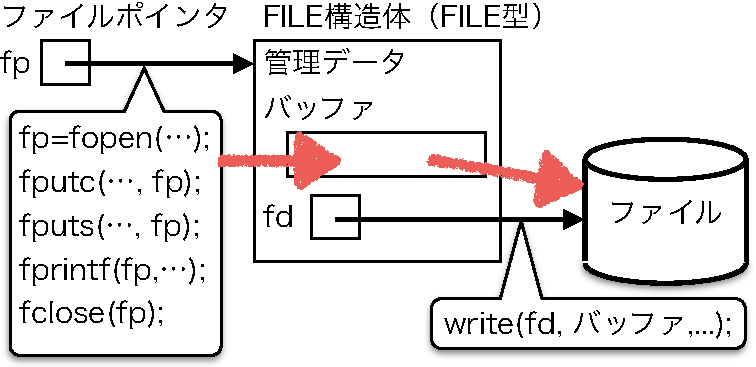
\includegraphics[scale=0.7]{Fig/HiVsLoWrite-crop.pdf}
\end{myfig}

\subsection{バッファの役割}
\figref{HiVsLoWrite}に示したように,
高水準I/O関数は出力データを FILE 構造体の内部にある{\em バッファ}に書き込む.
データはバッファがいっぱいになった時,
または,その他,一定の条件を満たした時に
\texttt{write()} システムコールによってファイルに書き込まれる.
これは FILE 構造体のバッファにデータをためることにより、
\texttt{write()} システムコールの実行回数を少なくする工夫である.
一般に{\em システムコールは重い処理}なので,
システムコールの実行回数が少なくなるような工夫が必要とされる
\footnote{\texttt{read()},\texttt{write()}システムコールの重さは,
一度に扱うデータの量にあまり左右されない.回数が重要である.}.

\figref{HiVsLoRead}に入力の場合を示す.
入力でもシステムコールの回数が少なくなるようにバッファを使用する.
入力の場合は\texttt{read()} システムコールでデータをバッファーにまとめて読み,
\|fgetc()| 等がバッファから入力データを必要に応じて取り出す仕組みになっている.

\begin{myfig}{btp}{高水準と低水準の関係(読み込みの場合)}{HiVsLoRead}
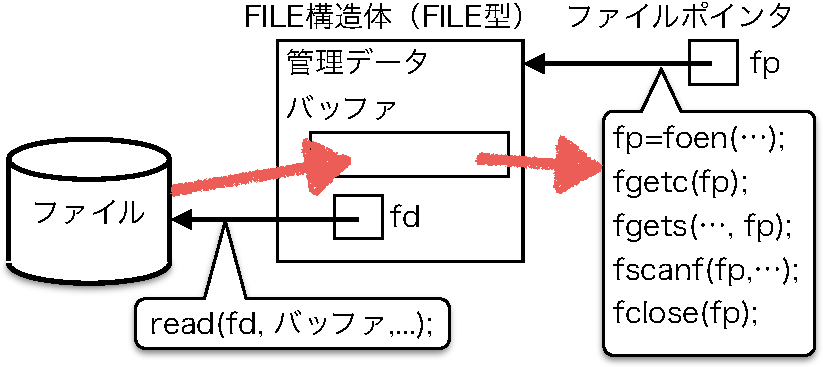
\includegraphics[scale=0.7]{Fig/HiVsLoRead-crop.pdf}
\end{myfig}

\section{標準入出力}
\|scanf()|,\|getchar()|,\|printf()|,\|putchar()|等は
引数にファイルポインタを持たない高水準I/O関数である.
プログラム実行開始時にオープンされたファイルポインタ\|stdin|や\|stdout|を,
これらは暗黙の内に使用する.
これらのファイルポインタを通して読み書きするデータの流れを
{\em 標準入出力ストリーム}と呼ぶ.
標準入出力ストリームの一覧と模式図を\tabref{stdio}と\figref{stdio}に示す.

\begin{mytable}{btp}{標準入出力ストリーム一覧}{stdio}
  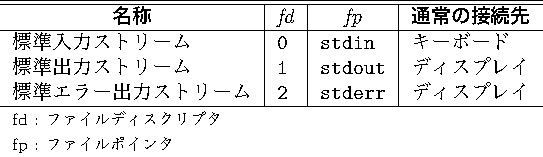
\includegraphics[scale=1.0]{Tbl/stdio.pdf}
\end{mytable}

\begin{myfig}{btp}{標準ストリームの構造}{stdio}
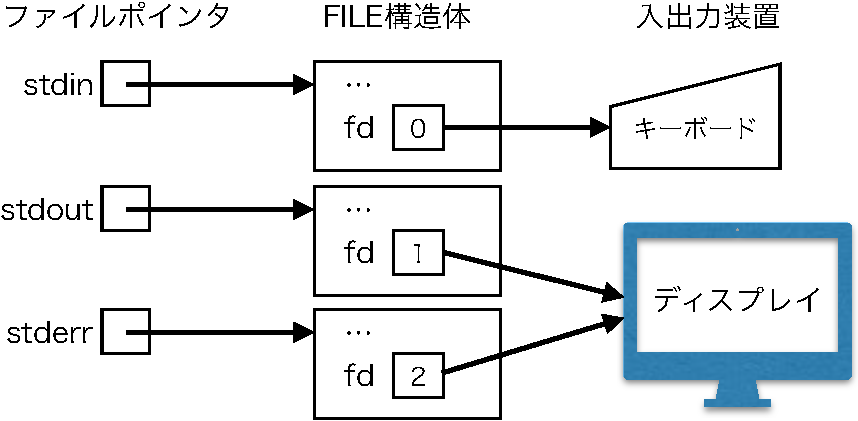
\includegraphics[scale=0.7]{Fig/stdio-crop.pdf}
\end{myfig}

\subsection{ユニファイドI/O}
標準入出力ストリームを使用する
\|scanf()|,\|getchar()|,\|printf()|,\|putchar()|等は,
ファイルポインタを引数に持つ
\|fscanf()|,\|fgetc()|,\|fprintf()|,\|fputc()|関数に
標準入出力ストリーム(\|stdin|,\|stdout|等)を渡した場合と同じ働きをする.
\tabref{printfVsFprintf}に同じ働きをする関数の対応を示す.
例えば\|getchar()|関数\footnote{正確には\texttt{getchar()}マクロ.}は,
\|fgetc()|の引数に標準入力ストリームを表す\|stdin|を
渡したものと同じ働きをする.

このようにファイルへの読み書きも,
キーボードやディスプレイ等の装置への入出力も,
ファイルポインタやファイルディスクリプタを用いて
同じ入出力関数や同じシステムコール(read/write)で行うことができる.
ファイルも装置も同様に(同じAPIで)扱う方式を{\em ユニファイドI/O}と呼ぶ.

\begin{mytable}{btp}{同じ役割をする入出力関数}{printfVsFprintf}
  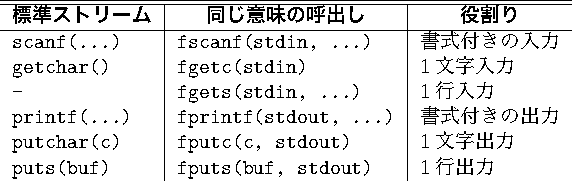
\includegraphics[scale=1.0]{Tbl/printfVsFprintf.pdf}
\end{mytable}

\subsection{標準入力ストリーム}
ファイルポインタ\|stdin|により参照され,
\|scanf()|や\|getchar()|等が暗黙に使用する入力ストリームである.
ファイルディスクリプタ 0 はプログラム起動前にオープンされている.
プログラムは起動時に\|FILE|構造体を作成し\figref{stdio}のように初期化する.

通常ファイルディスクリプタ 0 はキーホード用にオープンされるが,
ファイルにリダイレクトすることも可能である\footnote{
シェルで \texttt{<} を用いて
標準入力ストリームをファイルにリダイレクトすることができる.}.
リダイレクトはプログラムが起動される前にシェルによって行われる.

\subsection{標準出力ストリーム}
ファイルポインタ\|stdout|により参照され,
\|printf()|や\|putchar()|等が暗黙に使用する出力ストリームである.
ファイルディスクリプタ 1 はプログラム起動前にオープンされている.
プログラムは起動時に\|FILE|構造体を作成し\figref{stdio}のように初期化する.

通常ファイルディスクリプタ 1 はディスプレイ用にオープンされるが,
ファイルにリダイレクトすることも可能である\footnote{
シェルで \texttt{>} を用いて標準出力ストリームを
ファイルにリダイレクトすることができる.
}.

\subsection{標準エラー出力ストリーム}
ファイルポインタ\|stderr|により参照され,
エラーメッセージの出力用に使用するストリームである.
標準出力と標準エラー出力を分けることにより,
標準出力ストリームがファイルにリダイレクトされた場合でも,
エラーメッセージをディスプレイに表示できる.
\|stderr|は,エラーメッセージが遅延なく表示されるように.
\emph{バッファリング}\footnote{バッファにデータをためること.}を行わない.

ファイルディスクリプタ 2 はプログラム起動前にオープンされている.
プログラムは起動時に\|FILE|構造体を作成し\figref{stdio}のように初期化する.
ファイルディスクリプタ 2 もファイルにリダイレクトすることが可能であるが,
エラーメッセージが表示されなくなるので注意が必要である.

\section{実装例}
\cmm 言語の高水準I/Oの実装例が,
\url{https://github.com/tctsigemura/C--/blob/v3.1.12/lib/stdio.cmm}
(\cmm 言語で記述された約400行のプログラム)
に公開してある.
興味のある人は,周辺のプログラムも含めて読んで欲しい.

\section{低水準・高水準の性能比較}
システムコールを直接使用する低水準I/Oは,
上手にプログラミングすれば最高の性能を出すことができるが,
下手な使い方をすると全く性能が出ない.
一方で,高水準I/Oは自動的な\emph{バッファリング}を行うので,
誰が使用しても「ほどほど」の性能が出る.
以下では,高水準I/Oを用いたファイルコピーコマンドと,
低水準I/Oを用いたファイルコピーコマンドとの性能比較を行う.
なお,以下は macOS 10.13 での実行例である.

\begin{enumerate}
\item プログラムを準備する  \\
3年次に作成した高水準I/Oを用いたファイルコピーコマンドを
\texttt{mycp} という名前で準備する.
前回,作成した低水準I/Oを用いたファイルコピーコマンドで
バッファサイズを1バイト(1B)にしたものを
\texttt{mycp2\_1} という名前で準備する.
バッファサイズを1,024バイト(1KiB)のものを
\texttt{mycp2\_1024} という名前で準備する.

\item 大きめのファイルを作る \\
以下のような操作を行う.
この例では,
「デタラメな内容の特殊なファイル\texttt{/dev/urandom}から
1,024バイト(1KiB)ずつデータを読み込み
\texttt{aaa} と言う名前のファイルに
1,024バイト(1KiB)ずつ書き込む操作」を10,240回繰り返している.
その結果, \texttt{aaa} と言う名前で,
大きさが10MiB($10MiB = 1KiB \times 10Ki$)の内容がデタラメなファイルができる.

\lstinputlisting[language=bash,numbers=none]{Lst/dd_10M.txt}

\item 実行時間の測定方法 \\
time コマンドを用いて実行時間を測定する.
time コマンドは引数に渡されたコマンドを実行し,
実行中にユーザプログラムが費やした時間(user),
OSカーネルが費やした時間(system),
実際の実行時間(total)を表示する.

\texttt{mycp2\_1} を用いてファイル\texttt{aaa }を\texttt{bbb}にコピーする
時間を測定した例を次に示す.
実行時間が非常に短い場合は,
コピープログラムにバグがあり何もしていない可能性があるので注意すること.

\lstinputlisting[language=bash,numbers=none]{Lst/mycp2_1.txt}

\item 実行時間の測定 \\
上の方法で,\texttt{mycp},\texttt{mycp2\_1},
\texttt{mycp2\_1024}の三つのプログラムについて5回測定\footnote{
1回目はイレギュラーなデータが出やすいので,
実際には6回実行して1回目以外で測定する.
}を行い平均を求める.
5回の平均を求めるのは測定値が誤差を含んでいるからである.
なお,実行時間が長すぎて測定が困難な場合はファイルサイズを小さくしても良い.
\end{enumerate}

\section*{課題 No.2 }
上記の性能比較を実際に行う.
提出物は以下の通りとする.

\begin{enumerate}
\item 三つのプログラムについて実行時間を整理したもの
\item 使用したプログラムのソースコード
\item 感想・考察(ソースコードの余白に記入する)
\end{enumerate}

参考に,高水準版のファイルコピープログラムをリスト\ref{mycp}に掲載する.

\newpage

\lstinputlisting
    [float=btp,
      language=C,numbers=none,caption=高水準I/Oを使用したmycp,label=mycp]
    {Lst/mycp.c}

 % 高水準入出力と低水準入出力
\setcounter{page}{23}               % 授業で配布した時とページがずれたので
\chapter{ファイルシステム}
ファイルは二次記憶装置\footnote{
ハードディスク,USBメモリ,メモリカード,CD-ROM,SSD,磁気テープ等の
外部記憶装置(補助記憶装置)のこと.
通常これらは不揮発性であり,電源を切ってもデータが失われることはない.}
に格納された不揮発性のデータ記憶のことである.
通常,一台の二次記憶装置には多数のファイルが記憶される.
ファイルシステムとは,
多数のファイルを二次記憶装置に記憶し管理するために実装された仕組みや,
管理されているファイルの集合のことである.

ここでは,UNIXファイルシステムを例に,
ユーザから見たファイルシステムの構造や仕組みを紹介する.
WindowsやmacOS\footnote{macOSはUNIXの一種と考えてもよい.
}等のファイルシステムも,
基本的な考え方はUNIXと共通である.

%----------------------------------------------------------------------------
\section{ファイル木}
\figref{filesystem}にユーザから見たUNIXファイルシステムの構造を示す.
ファイルはディレクトリ(フォルダ)により階層的に管理されている.
ディレクトリとファイルからなる\figref{filesystem}のような構造を
ファイル木(ファイルツリー)と呼ぶ.

\begin{myfig}{btp}{ユーザから見たUNIXファイルシステムの構造}{filesystem}
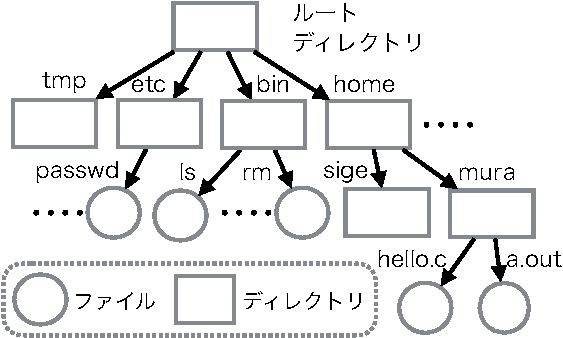
\includegraphics[scale=1.0]{Fig/FileSystem-crop.pdf}
\end{myfig}

ファイル木はルートディレクトリを根(ルート)とする有向の木構造\footnote{
グラフ理論の木構造と似ているが閉路を許す場合もある.}である.
木構造の節点(ノード)はディレクトリであり,葉(リーフ)はファイルである.
有向枝(エッジ)はリンクとも呼ばれる.
リンクには必ず名前が付けられている.
\emph{ファイルの本体とリンクは独立している.}
なお,UNIXファイルシステムではディレクトリもファイルの一種と考える.

%----------------------------------------------------------------------------
\section{特別なディレクトリ}
\figref{filesystem2}に特別なディレクトリを意識して書き直した
ファイル木の一部を示す.
細部にこだわって描いた\figref{filesystem2}は木構造と呼ぶには相応しくないが,
UNIXファイルシステムの実装をより忠実に表現している.

\subsection*{親ディレクトリ}
ファイルやディレクトリから見て根に近い側にあるディレクトリを
親ディレクトリと呼ぶ.
親ディレクトリの名前は「\texttt{..}」である.
\figref{filesystem2}では「\texttt{..}」と名付けたリンクで表現している\footnote{
UNIXファイルシステムには実際に「\texttt{..}」リンクを表現する
データが格納されている.}.

\subsection*{カレントディレクトリ}
ファイルシステム内でのユーザの現在位置をカレントディレクトリと呼ぶ.
カレントディレクトリの名前は「\texttt{.}」である.
\figref{filesystem2}では「\texttt{.}」と名付けたリンクで表現している\footnote{
UNIXファイルシステムには「\texttt{.}」リンクを
表現するデータも格納されている.}.

\subsection*{ルートディレクトリ}
ファイル木の根をルートディレクトリと呼ぶ.
ルートディレクトリの名前は「\texttt{/}」である.
ルートディレクトリには親ディレクトリが存在しないので,
\figref{filesystem2}では自身を親ディレクトリとしている.

\begin{myfig}{btp}{詳しいファイルシステムの構造}{filesystem2}
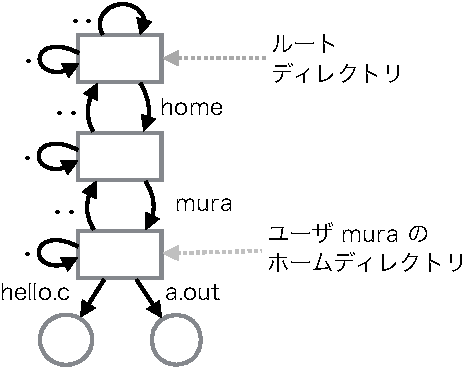
\includegraphics[scale=1.0]{Fig/FileSystem2-crop.pdf}
\end{myfig}

\subsection*{ホームディレクトリ}
ユーザがシステムにログインした時のデフォルトのカレントディレクトリを
ホームディレクトリと呼ぶ.
ホームディレクトリの位置はUNIXシステムの管理者が自由に決められる.
\figref{filesystem2}のように\texttt{/home}ディレクトリに
ユーザ名と同じ名前のディレクトリ準備し,ホームディレクトリにすることが多い
\footnote{macOSでは,\texttt{/Users} ディレクトリに作られる.}.

多くのUNIXツールではホームディレクトリのことを「\texttt{$\sim$}」と表記できる.
しかし,これはUNIXファイルシステムの機能ではない.
単にツールが内部で名前の置換えを行ってるだけである.

%----------------------------------------------------------------------------
\section{パス}
ファイル(ディレクトリも含む)は,
あるディレクトリからそのファイルへの通り道であるパス(path)により特定できる.
パスはファイル木のリンクに付いた名前を
「\texttt{/}」で区切って書いた文字列として表現する.
例えば\figref{filesystem}右下の\texttt{hello.c}ファイルは,
ルートディレクトリを起点とするパス\texttt{/home/mura/hello.c}で特定できる.
同じファイルを\texttt{/home/sige/../mura/./hello.c}でも特定できる.

\subsection*{絶対パス}
パスの先頭にある「\texttt{/}」はルートディレクリを表し,
「\texttt{/}」で始まるパスは絶対パスと呼ばれる.
絶対パスはルートディレクトリを起点にしたパスである.
上記の\texttt{/home/mura/hello.c}等は絶対パスの例である.

\subsection*{相対パス}
「\texttt{/}」以外で始めたパスは相対パスと呼ばれる.
相対パスはカレントディレクトリを起点にしたパスである.
例えばカレントディレクトリが\texttt{/home}ディレクトリの時,
\figref{filesystem}右下の\texttt{hello.c}ファイルは,
相対パス\texttt{mura/hello.c}で特定できる.
カレントディレクトリが\texttt{/home/sige}ディレクトリの時は,
相対パス\texttt{../mura/hello.c}で特定できる.

%----------------------------------------------------------------------------
\section{カレントディレクトリの変更と確認}
UNIXではプロセス(実行中のプログラム)毎にカレントディレクトリがある.
プロセスのカレントディレクトリを変更しても
他のターミナルやアプリに影響を与えないし,
次回のログインに引継がれることもない.

\subsection*{cdコマンド}
カレントディレクトリはcdコマンドで変更できる.

\begin{lstlisting}[numbers=none]
$ cd パス     # パスのディレクトリへ移動する
\end{lstlisting}

\subsection*{pwdコマンド}
カレントディレクトリのパスはpwdコマンドで確認できる.

\begin{lstlisting}[numbers=none]
$ pwd         # カレントディレクトリのパスを表示する
\end{lstlisting}

ファイルシステムが\figref{filesystem}の状態の時,
muraユーザがcd,pwdコマンドを操作した例をリスト\ref{cdpwd}に示す.
なお,muraユーザのホームディレクトリは\texttt{/home/mura}とする.

\lstinputlisting[float=btp,numbers=none,
  caption=cd,pwdコマンドの実行例,label=cdpwd]
                {Lst/cdpwd.txt}

%----------------------------------------------------------------------------
\section{リンク}
ファイルを別名(別パス)で指定できると便利なことがある.
UNIX ファイルシステムはファイルに別名を付ける方法を二つ準備している.

\subsection{ハードリンク}
これまでの例では一つのファイルに付き一つのリンクしか存在しなかったが,
本来はいくつあっても構わない\footnote{
グラフ理論の木構造とはかけ離れていくが。。。}.
このリンクのことを後に出てくるシンボリックリンクと区別するために
ハードリンクと呼ぶ\footnote{
単にリンクと呼ぶ時はハードリンクのことを指している.}.
\texttt{hello.c}ファイルに新たに二つリンクを追加した例を\figref{link}に示す.

ディレクトリは\emph{リンクを格納する特殊なファイル}である.
一つのディレクトリにいくつでもリンクを格納することができる.
また,最初から存在したリンクと後で追加したリンクの間に優劣はない.

\begin{myfig}{btp}{複数のリンクを持つファイル}{link}
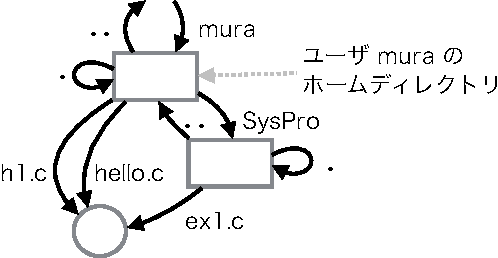
\includegraphics[scale=1.0]{Fig/Link-crop.pdf}
\end{myfig}

\subsection*{リンクの追加}
リンクの追加は次のコマンドで行う.

\begin{lstlisting}[numbers=none]
$ ln ファイルへのパス 追加するリンクのパス
\end{lstlisting}

\figref{filesystem2}の状態に二つのリンク\texttt{h1.c},\texttt{ex1.c}を追加し,
\figref{link}の状態に変える手順は次の通りである.
なお,リンク\texttt{ex1.c}を追加するより前に
\texttt{SysPro}ディレクトリを作っておく必要がある.

\lstinputlisting[numbers=none,float=ht]{Lst/ln.txt}

\subsection*{リンクの削除}

リンクの削除は rm コマンドで行う.

\begin{lstlisting}[numbers=none]
$ rm ファイルへのパス
\end{lstlisting}

rm コマンドはファイルを削除するコマンドと考えてきたが,
正確にはリンクを削除するコマンドである.
リンクを削除した結果,リンクを一つも持たなくなったファイル本体は削除される.
\emph{このようにリンクとファイル本体は別のものである.}
\figref{link}の状態から\figref{filesystem2}の状態に戻す手順を次に示す.

\lstinputlisting[numbers=none,float=ht]{Lst/lnrm.txt}

\subsection{シンボリックリンク}
シンボリックリンク\footnote{
シンボリックリンクのことをソフトリンクと呼ぶこともある.}
はパス(文字列)を格納した特殊なファイルである.
オペレーティングシステムがパスを解析する途中でシンボリックリンクを見つけると,
パス中のシンボリックリンク名をシンボリックリンクの内容で置き換えてから
パスの解析を続ける.
ハードリンクは同一の二次記憶装置内のファイルしかリンクできないが,
シンボリックリンクにはこのような制約はない.

シンボリックリンクにはどんなパスでも書き込むことができる.
まずリンク切れのシンボリックを作っておき,
後にファイル本体を作ることも許される.
一方でリンク先のファイルが削除された場合はリンク切れ状態になる.
これを応用すると,
置き換わったファイルを同じシンボリックリンクで参照し続けることができる.
\emph{リンク先ファイルが置換わることがシンボリックリンクの特徴である.}

\subsection*{シンボリックリンクの使用例}
\figref{symlink}にシンボリックリンクを使用した例を示す.
この例は\figref{link}のハードリンクをシンボリックリンクに置き換えたものである.
この図では,シンボリックリンクを内部にパスを書いた長方形で表現している.
シンボリックリンクもファイルの一種なので,
ディレクトリからハードリンクによって接続されている.

ユーザ mura のホームディレクトリからの相対パス\|h1.c|を用いてファイルを
指定した場合,パスはシンボリックリンクの内容と置き換えられ\|hello.c|になる.
同様に相対パス\|SysPro/ex1.c|は,\|ex1.c|がシンボリックリンク名なので
\|SysPro/../hello.c|に置き換えられる.
どちらの場合もホームディレクトリ直下の\texttt{hello.c}ファイルを
指定したことになる.

\begin{myfig}{btp}{シンボリックリンク}{symlink}
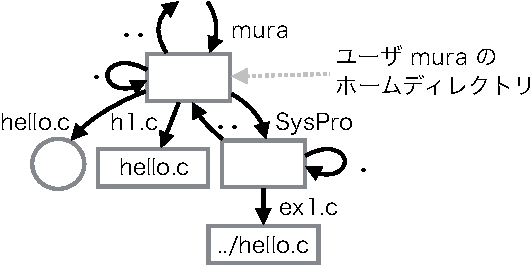
\includegraphics[scale=1.0]{Fig/SymLink-crop.pdf}
\end{myfig}

\subsection*{シンボリックリンクの作成}
シンボリックリンクは
\texttt{ln}コマンドに\texttt{-s}オプションを付けたものを用いて作成する.

\begin{lstlisting}[numbers=none]
$ ln -s リンクに書込むパス 作成するリンクのパス
\end{lstlisting}

\figref{filesystem2}の状態に
二つのシンボリックリンク\texttt{h1.c},\texttt{ex1.c}を追加し,
\figref{symlink}の状態に変える手順は次の通りである.
シンボリックリンク\texttt{ex1.c}に書込むパスは\|../hello.c|になる.
\emph{シンボリックリンクに書込むパスには
シンボリックリンクが存在するディレクトリからの相対パスを用いる\footnote{
絶対パスを書込むことも可能であるが普通は相対パスを用いる.
例えばシステム管理者がユーザ\texttt{mura}のホームディレクトリの
位置を変更しても,相対パスを用いておけばリンク切れにならない.}.}

\lstinputlisting[numbers=none]{Lst/lns.txt}

\subsection*{シンボリックリンクの削除}

シンボリックリンクの削除も\texttt{rm}コマンドで行う.

\begin{lstlisting}[numbers=none]
$ rm シンボリックリンクのパス
\end{lstlisting}

\figref{symlink}の状態から\figref{filesystem2}の状態に戻す手順を次に示す.

\lstinputlisting[numbers=none,float=ht]{Lst/lnsrm.txt}

%----------------------------------------------------------------------------
\section{ファイルの属性}
UNIXの各ファイル\footnote{ディレクトリやシンボリックリンクも含む}は,
ファイル本体にデータだけでなく幾つかの属性情報(メタデータ)を持っている.
ファイル名を属性情報の一部にしているOSも多いが,
UNIXではファイル名はファイル本体ではなくリンクに付属するので
属性に含まれていない.

\subsection{主な属性}
UNIXで用いられる主な属性情報は次の通りである.
これらは\texttt{stat}コマンドや\texttt{ls}コマンドで表示できる.

\begin{description}
\item[種類] 普通のファイル,ディレクトリ,シンボリックリンク等の区別.
\item[保護モード] openシステムコールで紹介した\texttt{rwxrwxrwx}.
\item[リンク数] ファイルを指しているハードリンクの数.
リンク数が0になるとファイル本体が削除される.
(例えば,\figref{link}の\texttt{hello.c}ファイルの場合は3になる)
\item[所有者] 所有者のユーザ番号.
\item[グループ] 属するグループのグループ番号.
\item[ファイルサイズ] ファイルの大きさ(バイト単位).
\item[最終参照日時] 最後にアクセスした時刻.
\item[最終変更日時] 内容を最後に変更した時刻.
\item[最終属性変更時刻] 属性を最後に変更した時刻.
\end{description}

\subsection{属性の表示方法}
属性を表示する専用コマンドは stat であるが,
ここでは,より手軽に使用できる ls コマンドを紹介する.
ls コマンドは\texttt{-l}オプションを付けて実行すると,
ファイルの属性情報の一部を表示する\footnote{
より多くの属性情報を知りたい時は,stat コマンドを用いる.}.
以下に ls コマンドを実行した例を示す.

\begin{lstlisting}[numbers=none]
$ ls -l a.txt
-rw-r--r--  1 mura  staff 10 May  1 18:18 a.txt
\end{lstlisting}

実行例の表示は以下の意味を持っている.

\begin{description}
\item[ファイルの種類] 一文字目の「\texttt{-}」は
ファイルが普通のファイルであることを表している.
一文字目が「\texttt{d}」はディレクトリであること,
「\texttt{l}」はシンボリックリンクであることを表す.
\item[ファイルの保護モード] openシステムコールで紹介したもの
(\texttt{rwxrwxrwx}).
\item[リンク数] \texttt{1}はリンク数が1であることを表している.
\item[所有者] \texttt{mura}は
ファイルの所有者がユーザ mura であることを表している.
メタ情報の内部表現はユーザ番号であるが,
ls コマンドがユーザ名に変換して表示している.
\item[グループ] \texttt{staff}は
ファイルがグループ staff に属することを表している.
メタ情報の内部表現はグループ番号であるが,
ls コマンドがグループ名に変換して表示している.
\item[ファイルサイズ] \texttt{10}はファイルのサイズが10バイトで
あることを表している.
\item[最終変更日時] \texttt{May 1 18:18} はファイルの最終変更日時である.
\item[パス] \texttt{a.txt} はファイルへ到達するために使用したパスである.
\emph{パス名(ファイル名)はファイルの属性ではない.}
\end{description}

\subsection{属性の変更方法}
ファイルの保護モードは一般ユーザも変更する機会が多い.
ファイルの保護モードの変更には chmod コマンドを用いる.
以下に書式を,リスト\ref{lstchmod}に使用例を示す.

\begin{lstlisting}[numbers=none]
$ chmod OOO ファイル...      # 書式1
$ chmod ugo+rwx ファイル...  # 書式2
$ chmod ugo-rwx ファイル...  # 書式3
\end{lstlisting}

\begin{description}
\item[書式1] \texttt{OOO}は3桁の8進数である.
8進数で保護モードを指定する.
8進数の値はopenシステムコールの書式2と同じである.

\item[書式2,3] \texttt{ugo+-rwx}の文字を組合せて
保護モードの変更方法を記述する.
各文字の意味は\tabref{chmod}の通りである。
例えば,
所有者とグループに書込み権と実行権を与える場合なら\texttt{ug+wx}のように書く.
その他のユーザの読出し権を取上げるなら\texttt{o-r}のように書く.
\end{description}

以下に chmod コマンドの使用例を示す.

\begin{mytable}{btp}{\texttt{chmod}コマンドの引数の意味}{chmod}
  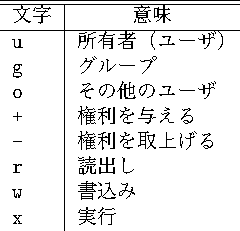
\includegraphics[scale=1.0]{Tbl/chmodOptions.pdf}
\end{mytable}

\lstinputlisting[float=btp,numbers=none,
  caption=chmodコマンドの使用例,label=lstchmod]{Lst/chmod.txt}

\newpage
\section*{課題 No.3}
以下を行い,それに用いた手順と結果を印刷して提出しなさい.

\begin{enumerate}
\item パスとハードリンク
\begin{enumerate}
\item 自分のホームディレクトリのパスを調べる.
\item ハードリンクに関する課題を行うために,
ディレクトリ\texttt{/tmp}にカレントディレクトリを移動する\footnote{
PC教室のMacは一般ユーザのホームディレクトリを共有ドライブ上に置いている.
macOSの共有ドライブ上にはハードリンクを作ることができない.
\texttt{/tmp}はローカルハードディスク上にあり,かつ,
誰でも自由に一時的なファイルを作ることができるディレクトリである.}.
\item \texttt{/tmp}以下に\figref{link}のディレクトリやファイルを作る.
\item \texttt{ls -l}を用いてファイルの種類やリンク数を確認する.
\item 相対パスを用いて\texttt{hello.c}の内容を表示する.
(表示には\texttt{cat}コマンドを用いると良い.)
\item 絶対パスを用いて\texttt{hello.c}の内容を表示する.
\item \texttt{h1.c}を利用した相対パスを用いて\texttt{hello.c}の内容を表示する.
\item \texttt{ex1.c}を利用した相対パスを用いて
\texttt{hello.c}の内容を表示する.
\item カレントディレクトリを\texttt{SysPro}に変更する.
\item \texttt{ex1.c}を利用した相対パスを用いて
\texttt{hello.c}の内容を表示する.
\item \texttt{hello.c}を利用した相対パスを用いて
\texttt{hello.c}の内容を表示する.
\item ディレクトリのハードリンクができるか試す.
\item 課題のために作成したファイルやディレクトリを全て削除する.
\end{enumerate}

\item シンボリックリンク
\begin{enumerate}
\item シンボリックリンクを作ってみる.
\item シンボリックリンクを\texttt{ls -l}を用いて確認する.
\item シンボリックリンクを用いてファイルをアクセスできることを確認する.
\item リンク切れのシンボリックリンクを使用するとどうなるか確認する.
\item ディレクトリに対するリンクを作って使用できることを確認する.
\item 他のディレクトリにあるファイルをリンクして使用できることを確認する.
\item シンボリックリンクのループを作る.(a.txt →  b.txt,b.txt →  a.txt)
\item ループしているシンボリックリンクを使用するとどうなるか確認する.
(\|$ cat a.txt|)
\end{enumerate}

\item 保護モード
\begin{enumerate}
\item テキストファイル(\texttt{hello.c})と
実行可能ファイル(\texttt{a.out})を準備する.
\item \texttt{chmod}で保護モードを変化させてみる.
\item \texttt{ls -l}で変化を確認する.
\item 保護モードを変化させて,ファイルの読出しや実行ができるか確認する.
\item ディレクトリの保護モードは何の意味を持つか考える.
\end{enumerate}
\end{enumerate}
 % ファイルシステム
\chapter{ファイル操作システムコール}

この章ではファイルを操作するシステムコールの中で重要なものについて学ぶ.
前の章で使用したユーティリティコマンド(ln, rm, chmod 等)が
内部で使用しているシステムコールである.

%==============================================================================
\section{unlink システムコール}
ファイルを削除するシステムコールである.
rm コマンドは,このシステムコールを利用している.
「ファイルの削除」は正確にはリンク(名前)の削除の意味である.
ファイルはリンクを一つも持たなくなった時に削除される.
シンボリックリンク等の削除にも使用できるが,
ディレクトリの削除には使用できない.

\begin{description}
\item[書式] \|path|引数でリンクのパスを一つ指定する.
\begin{lstlisting}[numbers=none]
  #include <unistd.h>
  int unlink(char *path);
\end{lstlisting}

\item[解説] uninkシステムコールを使用するプログラムは
\|unistd.h|をインクルードする必要がある.
unlink システムコールは,正常時に 0 ,エラー発生時に -1 を返す.
エラー原因は\|perror()|関数で表示できる.

\item[引数] \|path|は削除するリンク(ファイル)のパスを表す文字列である.

\item[使用例] \|"a.txt"|ファイルを削除する例を示す.
\begin{lstlisting}[numbers=none]
  // ファイルの削除
  if (unlink("a.txt")<0) {   // "a.txt" 削除
    perror("a.txt");         // エラー原因表示
    exit(1);                 // エラー終了
  }
\end{lstlisting}
\end{description}

%==============================================================================
\section{mkdirシステムコール}
ディレクトリ(フォルダ)作成するシステムコールである.
mkdirコマンドは,このシステムコールを使用している.

\begin{description}
\item[書式] \|path|,\|mode|の二つの引数で新規ディレクトリのパスと
保護モードを指定する.
\begin{lstlisting}[numbers=none]
  #include <sys/stat.h>
  int mkdir(char *path, int mode);
\end{lstlisting}

\item[解説] mkdirシステムコールを使用するプログラムは
\|sys/stat.h|をインクルードする必要がある.
mkdir システムコールは,正常時に 0 ,エラー発生時に -1 を返す.
エラー原因は\|perror()|関数で表示できる.
mkdir システムコールはパスに含まれる途中のディレクトリは作らない.
途中のディレクトリは予め作成しておく必要がある.

\item[引数] \|path|は新規作成するディレクトリのパス,
\|mode|は新しいディレクトリの保護モード(\|rwxrwxrwx|)である.

\item[使用例] \|"newdir"|ディレクトリを作成する例である.
\begin{lstlisting}[numbers=none]
  // ディレクトリの作成
  if (mkdir("newdir", 0755)<0) {   // "newdir" を rwxr-xr-x で作成
    perror("newdir");              // エラー原因表示
    exit(1);                       // エラー終了
  }
\end{lstlisting}
\end{description}

%==============================================================================
\section{rmdir システムコール}
ディレクトリを削除するシステムコールである.
rmdir コマンドは,このシステムコールを利用している.
\emph{空でないディレクトリを削除することはできない.}

\begin{description}
\item[書式] \|path|引数でディレクトリのパスを一つ指定する.
\begin{lstlisting}[numbers=none]
  #include <unistd.h>
  int rmdir(char *path);
\end{lstlisting}

\item[解説] rmdirシステムコールを使用するプログラムは
\|unistd.h|をインクルードする必要がある.
rmdirシステムコールは,正常時に 0 ,エラー発生時に -1 を返す.
エラー原因は\|perror()|関数で表示できる.

\item[引数] \|path|は削除するディレクトリのパスである.

\item[使用例] \|"newdir"|と名付けられたディレクトリを削除する例である.
\begin{lstlisting}[numbers=none]
  // ディレクトリの削除
  if (rmdir("newdir")<0) {  // "newdir" 削除
    perror("newdir");       // エラー原因表示
    exit(1);                // エラー終了
  }
\end{lstlisting}
\end{description}

%==============================================================================
\section{link システムコール}
リンク(ハードリンク)を作成するシステムコールである.
ln コマンドは,ハードリンクを作るとき,このシステムコールを利用している.

\begin{description}
\item[書式] 既に存在するリンクのパスと
新しく作るリンクのパスを指定する.
\begin{lstlisting}[numbers=none]
  #include <unistd.h>
  int link(char *oldpath, char *newpath);
\end{lstlisting}

\item[解説] link システムコールを使用するプログラムは
\|unistd.h|をインクルードする必要がある.
link システムコールは,正常時に 0 ,エラー発生時に -1 を返す.
エラー原因は\|perror()|関数で表示できる.

\item[引数] \|oldpath|はもともと存在するリンクを表すパス,
  \|newpath|は新しく作るリンクのパスである.

\item[使用例1] ファイルにリンク\|"b.txt"|を追加する例である.
\begin{lstlisting}[numbers=none]
  // ハードリンクの作成
  if (link("a.txt", "b.txt")<0) { // リンク"b.txt"を作る
    perror("link");               // "a.txt"と"b.txt"のどちらが原因か不明なので
    exit(1);                      // エラー終了
  }
\end{lstlisting}

\item[使用例2]unlinkシステムコールと組合せて
ファイルの移動(ファイル名の変更)に応用した例である.
リンク\|"a.txt"|で参照されていたファイルは,
リンク\|"b.txt"|で参照されるように変更される.
\begin{lstlisting}[numbers=none]
  unlink("b.txt");                // 念のため"b.txt"を消す(エラーは無視)
  if (link("a.txt", "b.txt")<0) { // リンク"b.txt"を作る
    ... エラー処理 ... 
  }
  if (unlink("a.txt")<0) {        // リンク"a.txt"を消す.
      ... エラー処理 ... 
  }
\end{lstlisting}
\end{description}

%==============================================================================
\section{symlink システムコール}

シンボリックリンクを作成するシステムコールである.
ln コマンドは,シンボリックリンクを作るとき(\|-s|オプション使用時),
このシステムコールを利用している.

\begin{description}
\item[書式] 新規作成するシンボリックリンクのパスと,
シンボリックリンクに書き込むパスを指定する.
\begin{lstlisting}[numbers=none]
  #include <unistd.h>
  int symlink(char *path1, char *path2);
\end{lstlisting}

\item[解説] symlink システムコールを使用するプログラムは
\|unistd.h|をインクルードする必要がある.
symlink システムコールは,正常時に 0 ,エラー発生時に -1 を返す.
エラー原因は\|perror()|関数で表示できる.

\item[引数] \|path1|はシンボリックリンクに書き込むパスである.
\|path2|は新規に作成するシンボリックリンク自身のパスである.

\item[使用例] 内容が\|"a.txt"|のシンボリックリンクを
\|"b.txt"|という名前で作る.
シンボリックリンクの内容はチェックされない(リンク切れ状態でも良い)ので,
エラーが発生した場合,原因は\|"b.txt"|である.
エラーメッセージには\|"b.txt"|を含める.
\begin{lstlisting}[numbers=none]
  // シンボリックリンクの作成
  if (symlink("a.txt", "b.txt")<0) { // リンク"b.txt"を作る
    perror("b.txt");                 // エラー原因は必ず"b.txt"
    exit(1);                         // エラー終了
  }
\end{lstlisting}
\end{description}

%==============================================================================
\section{rename システムコール}
ファイルの移動(ファイル名の変更)を行うシステムコールである.
mv コマンドは,このシステムコールを利用している.

\begin{description}
\item[書式] 新旧二つのパスを指定する.
\begin{lstlisting}[numbers=none]
  #include <stdio.h>
  int rename(char *from, char *to);
\end{lstlisting}

\item[解説] rename システムコールを使用するプログラムは
\|stdio.h|をインクルードする必要がある.
rename システムコールは,正常時に 0 ,エラー発生時に -1 を返す.
エラー原因は\|perror()|関数で表示できる.

\item[引数] \|from|は古いパス\|to|は移動後の新しいパスである.
\|from|で参照されていたファイルが\|to|で参照されるようになる.

\item[使用例] \|"a.txt"|のパスを\|"b.txt"|に変更する例である.
\begin{lstlisting}[numbers=none]
  // ファイルの移動
  if (rename("a.txt", "b.txt")<0) { // "a.txt" を "b.txt" に変更
    perror("rename");               // エラー原因がどっちのパスか不明
    exit(1);                        // エラー終了
  }
\end{lstlisting}
\end{description}

%==============================================================================
\section{chmod(lchmod)システムコール}
ファイルの保護モードを変更するシステムコールである.
chmod コマンドは,このシステムコールを利用している.

\begin{description}
\item[書式] ファイルのパスと新しい保護モードを指定する.
\begin{lstlisting}[numbers=none]
  #include <sys/stat.h>
  int chmod(char *path, int mode);
  int lchmod(char *path, int mode);
\end{lstlisting}

\item[解説] chmodシステムコールを使用するプログラムは
\|sys/stat.h|をインクルードする必要がある.
chmod システムコールは
\|path|で指定されるファイルの保護モードを変更する.
シンボリックリンクが指定された場合,
lchmod システムコールはシンボリックリンクが指すファイルではなく,
シンボリックリンクの保護モードを変更する.
chmod システムコールは,正常時に 0 ,エラー発生時に -1 を返す.
エラー原因は\|perror()|関数で表示できる.

\item[引数] \|path|は対象となるファイルのパスである.
\|mode|は新しい保護モード(\|rwxrwxrwx|)である.
保護モードの意味はopenシステムコールの章に解説がある.

\item[使用例] \|"a.txt"|の保護モードを\|rw-r--r--|に変更する例である.
\begin{lstlisting}[numbers=none]
  // ファイルモードの変更
  if (chmod("a.txt", 0644)<0) { // ファイル"a.txt"のモードをrw-r--r--に変更
    perror("a.txt");            // エラー原因を表示
    exit(1);                    // エラー終了
  }
\end{lstlisting}
\end{description}

%==============================================================================
\section{readlink システムコール}

readlink システムコールは
シンボリックリンクに書き込まれている内容(パス)を読み出す.
ls コマンドはシンボリックリンクの内容を表示するために,
このシステムコールを利用している.

\begin{description}
\item[書式] シンボリックリンクを示すパスと,内容を読み出すバッファを指定する.
\begin{lstlisting}[numbers=none]
  #include <unistd.h>
  int readlink(char *path, char *buf, int size);
\end{lstlisting}

\item[解説] readlinkシステムコールを使用するプログラムは
\|unistd.h|をインクルードする必要がある.
readlink システムコールは
\|path|で指定されるシンボリックの内容を\|buf|に読み出す.
\|path|はシンボリックリンクを示すものでなければならない.
readlink システムコールは,
正常時に読み出した文字数を,エラー発生時に-1を返す.
エラー原因は\|perror()|関数で表示できる.
読み出した文字列は\verb;'\0';で終端\emph{されない}ので注意を要する.

\item[引数] \|path|は目的のシンボリックリンクのパスである.
\|buf|は内容を読み出す領域(バッファ)のポインタ,
\|size|は領域のサイズである.

\item[使用例] シンボリックリンク\|"b.txt"|の内容を読み出し表示する例である.
読み出した文字列を\verb;'\0';で終端することを見越して,
バッファの大きさ(100)より小さい領域サイズ(99)を指定している.
\begin{lstlisting}[numbers=none]
  // シンボリックリンクの読み出し
  char *name = "b.txt";
  char buf[100];
  int n = readlink(name, buf, 99); // シンボリックリンクの内容をbufに読み出す
  if (n<0) {                       // エラーチェック
    perror(name);                  // エラー原因を表示
    exit(1);                       // エラー終了
  }
  buf[n]='\0';                     // C言語型の文字列として完成させる
  printf("%s -> %s\n", name, buf); // ls -l 風に表示
\end{lstlisting}
\end{description}

\begin{figure}
\begin{framed}
\subsection*{参考:strtol 関数}
chmod プログラムを作成するためには,
保護モードをコマンド行引数から入力する必要がある.

\centerline{書式: \texttt{chmod mode file ...}}

\|mode|を8進数で指定する場合,
8進数を表現する文字列から整数値(int 型)に変換しなければならない.
strtol 関数は8進数を整数値に変換するために使用できる.
簡易版の chmod プログラムを作るために必要な
strtol 関数の使用例を以下に示す.

(詳細はオンラインマニュアル「\|man 3 strtol|」で調べること.)

\begin{lstlisting}[numbers=none, frame=none]
#include <stdlib.h>
  ...
  char *ptr;
  char *ostr = argv[1];               // 入力の8進数文字列
  int mod;

  mod = strtol(ostr, &ptr, 8);        // 8進数文字列の値を整数で求める
  if (*ostr=='\0' || *ptr!='\0') {
    fprintf(stderr, "\'%s\' : 8進数の形式が不正\n", ostr);
    return 1;
  }
  printf("%d,%x,%o\n", mod, mod,mod); // 10進,16進,8進で表示
  ...

// 実行例
% ./a.out 777
511,1ff,777
\end{lstlisting}
\end{framed}
\end{figure}

\subsection*{課題 No.4}

\begin{enumerate}
\item 簡易版のUNIXコマンドを作成しなさい.

UNIXコマンド,rm,mkdir,rmdir,ln,mv,chmodの中から3つ以上を選択し,
上記のシステムコールを使用して簡易版を作ってみる.
使用方法のエラーチェック,システムコールのエラーチェックは行うこと.

\item 自分が作った簡易版と本物の機能の違いを調べる.

「\|% man 1 rm|\footnote{
オンラインマニュアル第1章「一般コマンド」の\texttt{rm}が表示される.
}」 等で本物のマニュアルを参照し比較してみる.

\item rename システムコールの必要性を考察する.

UNIXは Simple is best の思想で作られてきた.
既存の機能を組み合わせて実現できる場合は専用機能の追加はしないことが多い.
rename システムコールの機能は
link,unlink システムコールの組み合わせでも実現できるが,
なぜ追加されたか考えなさい.

\item stat システムコール,readdir 関数について調べてみる.

これらは何コマンドを作る時に必要になるか?
\end{enumerate}
 % ファイル操作システムコール
\chapter{プロセスとジョブ}

%==============================================================================
\section{プロセス}
皆さんは,これまでPCを使用してきた経験から,
\figref{pc}に示すように,
同時に複数のプログラムがPCで実行されていることを理解しているだろう.
また,同じプログラムが複数のウインドで同時に実行されることがある
ことも理解しているだろう\footnote{
\figref{pc}の例では二つのターミナル(Terminal)夫々の中で,
合計二つのa.outが同時に実行されている.
}.

つまり,一連の機械語命令である\emph{プログラム}だけでなく,
実行中のプログラムのインスタンスも意識する必要がある.
実行中のプログラムのインスタンスのことを\emph{プロセス}と呼ぶ.

\begin{center}
  \emph{\Large プロセス = 実行中のプログラム}
\end{center}

\begin{myfig}{btp}{PC上の複数プログラム}{pc}
  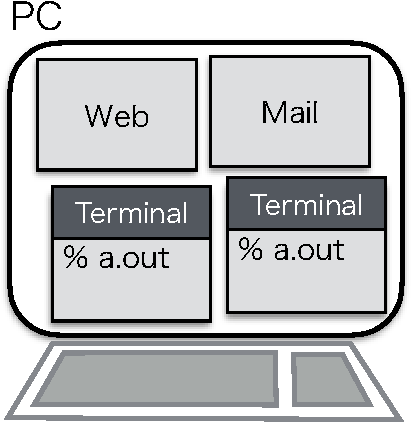
\includegraphics[scale=0.7]{Fig/pc-crop.pdf}
\end{myfig}

\subsection{プロセスの構造}

\figref{proc}にプロセスの構造を模式的に示す.
プロセスは,
プロセス名(プロセス番号)等の「プロセスの情報」や,
前回プロセスを実行中だった時の「CPUの状態」を保存する領域(仮想CPU)と
そのプロセス専用の「メモリ空間」(仮想メモリ)を持つ.
一つ一つのプロセスが一台のコンピュータに相当するるものを備えており,
プロセスを一台の\emph{仮想コンピュータ}と考えることもできる.

\begin{center}
\emph{\Large プロセス = 仮想コンピュータ}
\end{center}


\begin{myfig}{btp}{プロセスの構造}{proc}
  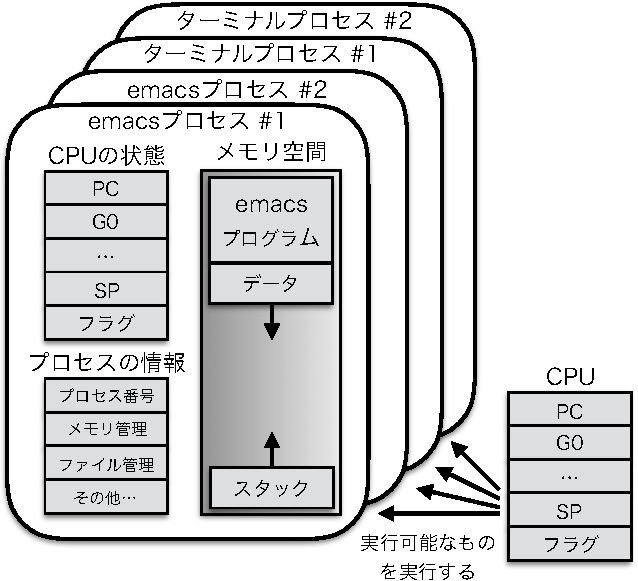
\includegraphics[scale=0.7]{Fig/proc-crop.pdf}
\end{myfig}

PC内には多数のプロセスが同時に存在し,
これらの中から実行可能なもの\footnote{
例えば,ユーザのキー操作待ちのものは実行不可能なプロセスである.}
を一つ\footnote{CPU(または,コア)が複数ある場合は一つとは限らない.}
選択し実物のCPU(実CPU)で実行する.
実行するプロセスを短時間に次々切替えることにより,
複数のプロセスが同時に実行されているように見せかけることもできる.

\subsection{プロセス関連のUNIXコマンド}

\subsubsection{psコマンド}
PC内で実行中のプロセスの一覧表を状態付きで表示するコマンドである.
macOSでターミナルを二つ開いた状態で,
一方のターミナルでvi(vim)を起動し,
もう一方のターミナルでpsコマンドを実行した例をリスト\ref{ps1}に示す.

\lstinputlisting[numbers=none,
  caption=psの実行例,float=btp,label=ps1]{Lst/ps.txt}

全てのプログラムはプロセスとして実行される.
ターミナルやpsコマンド自身もプロセスとして実行されるが,
macOSの標準では,これらは表示されない.
\texttt{-zsh} はターミナルに入力されたコマンドを解釈して実行するシェルである.
表示内容の意味は\tabref{psOut}\footnote{
リスト\ref{ps1}の実行例に含まれていない項目も含んでいる.}の通りである.

制御端末はプロセスがどのターミナルで実行されているかを示す.
ターミナルの名前はリスト\ref{ps1}の最後の部分のように,
ターミナルでtty コマンドを実行すると確認できる.

%\lstinputlisting[numbers=none,float=btp]{Lst/tty.txt}

\begin{mytable}{btp}{psコマンドの表示内容}{psOut}
  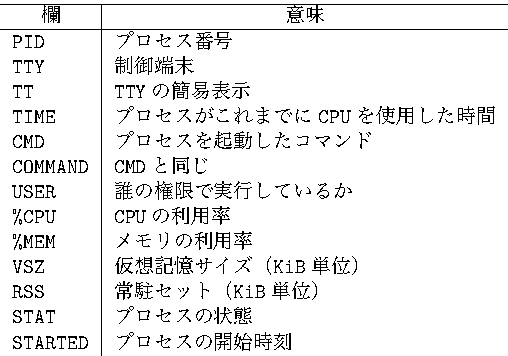
\includegraphics[scale=1.0]{Tbl/psOut.pdf}
\end{mytable}

\subsubsection{psコマンドのオプション}
\tabref{psOptions}にpsコマンドのオプションの一部を
\footnote{
最近のUNIXではオプションが大きく変更されている.
%詳しくは,各自で\texttt{man 1 ps}を用いて調べること.
%なお,macOSのpsでは古いオプションも使用できるので,
ここでは簡単で分かりやすい古いオプションの使用例を示す.
}
リスト\ref{ps2}にオプションを用いた時の実行例を示す.
\texttt{ps u}を実行するとリスト\ref{ps1}と同じ三つのプロセスに付いて,
より詳しい表示がされた.
表示内容の意味は\tabref{psOut}の通りである.
プロセスの状態は,\tabref{psStat}の二文字を組合せて表現される.
例えば,リスト\ref{ps2}で\texttt{vi}は\texttt{S+}なので,
フォアグラウンドで実行中に短期間のスリープをしていることが分かる.

\begin{mytable}{btp}{psコマンドのオプション(一部)}{psOptions}
  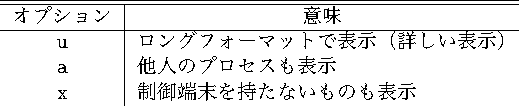
\includegraphics[scale=1.0]{Tbl/psOptions.pdf}
\end{mytable}

\lstinputlisting[numbers=none,caption=psコマンドのオプション付き実行例,
  float=btp,label=ps2]{Lst/psLong.txt}

\begin{mytable}{btp}{psコマンド\texttt{STAT}表示の意}{psStat}
  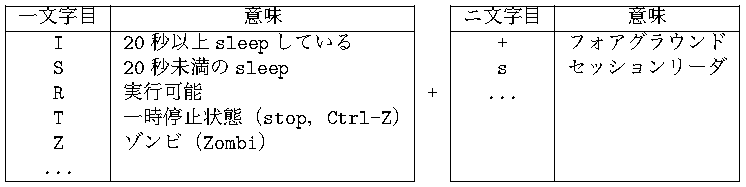
\includegraphics[scale=1.0]{Tbl/psStat.pdf}
\end{mytable}

\texttt{ps au}を実行すると\texttt{root}\footnote{
UNIX系のオペレーティングシステムでは,
システム管理者の名前が\texttt{root}である.}のプロセスも表示されている.
%\texttt{u}オプションも付けているので詳しい表示形式になっている.
この実行例では ps コマンド自身も表示されている.
ps コマンドは\texttt{root}のプロセスとして実行されていたことが分かる.

\texttt{ps aux}を実行すると全ユーザの全プロセスが表示される.
\texttt{TT}が「\texttt{??}」のプロセスが制御端末を持たないものである.
macOSでは色々な権限で600程度のプロセスが実行されていることが分かる.

\subsubsection{killコマンド}

プロセスにシグナル(ソフトウェア割込み)を送るコマンドである.
通常,プロセスは予期しないシグナルを受取ると終了する.
killコマンドはシグナル(省略可能)とプロセス番号を引数にする.
使用できるシグナルの一部を\tabref{kill}に,
使用例をリスト\ref{sleepKill}に示す\footnote{
コマンド行から簡単に起動できて,しばらく実行し続ける sleep を例にする.
}.

\begin{mytable}{btp}{\texttt{kill}コマンドのシグナル名と番号(一部)}{kill}
  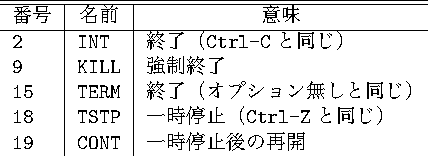
\includegraphics[scale=1.0]{Tbl/killOptions.pdf}
\end{mytable}

\lstinputlisting[numbers=left,caption=killコマンドの使用例,
  float=btp,label=sleepKill]{Lst/kill.txt}

%\begin{description}
%\item[1行] sleep をバックグラウンドで起動する.
%\item[2行] sleep はジョブ番号1,プロセス番号75868で起動した.
%\item[3行] ps コマンドで確認してみる.
%\item[7行] sleep にTERMシグナルを送信してみる.(シグナル名は省略)
%\item[8行] sleep は終了した.
%\item[9行] sleep を再度バックグラウンドで起動する.
%\item[11行] sleep にTSTPシグナルを送信してみる.
%\item[12行] sleep は一時停止した.
%\item[13行] sleep が存在し続けていることを確認する.
%\item[17行] sleep にCONTシグナルを送信してみる.(動き始めたはず)
%\item[18行] シグナル名を省略したのでTERMシグナルが送られたはず.
%\item[19行] sleep は終了した.
%\end{description}

%==============================================================================
\section{ジョブ}
ジョブはユーザの視点からはプロセスとよく似たものに見える.
ジョブはシェルが管理するプロセスのグループである.
シェルは一度に起動されたひとまとまりのプロセスを一つのジョブとして扱う.
リスト\ref{job}に例を示す.

\lstinputlisting[numbers=none,caption=ジョブの例,label=job,float=btp]
                {Lst/job.txt}

\subsection{ジョブの種類}
ジョブにはフォアグラウンド・ジョブとバックグラウンド・ジョブの2種類がある.
夫々、次のような特徴がある.実行例はリスト\ref{fgbg}の通りである.

\begin{description}
\item[フォアグラウンド・ジョブ]
シェルがジョブの終了を待つ.
%ジョブが
終了したらプロンプトが表示される.

\item[バックグラウンド・ジョブ]
コマンドの最後に\texttt{\&}を付けて実行する.
シェルがジョブの終了を待たない.
ジョブが終了していなくてもプロンプトが表示される.
次のジョブと並列実行ができる.
\end{description}

\lstinputlisting[numbers=none,caption=フォアグラウンド・バックグラウンド,
    float=btp,label=fgbg]{Lst/fgbg.txt}

\subsection{ジョブ制御}
シェルと制御端末はジョブに対して働きかけをすることができる.

\begin{description}
\item[Ctrl-C] フォアグラウンド・ジョブにINTシグナルを送る.
(通常,ジョブは終了する.)

\item[Ctrl-Z] フォアグラウンド・ジョブにTSTPシグナルを送る.
(ジョブは一時停止状態になる.)

\item[jobs] そのシェルが管理しているジョブの一覧を表示する.

\item[fg] バックグラウンド・ジョブや一時停止中のジョブを
フォアグラウンドに切替える.
ジョブ番号を指定することもできる.

\item[bg] 一時停止状態のジョブをバックグラウンドで再開する.
ジョブ番号を指定することもできる.
\end{description}

リスト\ref{jobControl}にジョブ制御の使用例を示す.

\lstinputlisting[numbers=left,caption=ジョブ制御の使用例,
  float=h,
  label=jobControl]{Lst/jobControl.txt}

%\begin{description}
%\item [1行] sleep をフォアグラウンドで起動する.
%\item [2行] Ctrl-Z で sleep へTSTPシグナルを送る.(sleepは一時停止状態になる)
%\item [4行] sleep をバックグラウンドで再開する.
%\item [6行] もう一つの sleep をバックグラウンドで起動する.
%\item [8行] 二つの sleep ジョブがあることを確認する.
%\item [10行] ジョブ 2 がカレントジョブ
%(ジョブを明示しないときの操作対象)である.
%\item [11行] 番号を明示してジョブ 1 をフォアグラウンドに変更する.
%\item [13行] Ctrl-C でジョブ 1 へINTシグナルを送る.(sleepは終了する)
%\item [14行] sleep ジョブが一つだけになっていることを確認する.
%\end{description}

%==============================================================================
%\section*{課題 No.5}
%\begin{enumerate}
%\item 本文と照らし合わせながらプロセスの
%実行例(リスト\ref{jobControl}まで)を試し,内容をよく理解しなさい.
%一時停止状態のsleepを操作するとどうなるか等,よく観察すること.
%
%\item 以下の操作方法を考えて手順を説明しなさい.
%
%\begin{enumerate}
%\item ターミナルが一つしか使用できない条件下で,
%フォアグラウンドで暴走してしまった(Ctrl-Cで終了しなくなった)
%ジョブを強制終了する手順.
%(KILLシグナルを使用すること)
%
%\item 間違ってフォアグラウンドで起動したsleepを
%バックグラウンドに変更する手順.
%
%\item バックグラウンドで実行中のジョブを
%フォアグラウンドに変更してCtrl-Cで終了する手順.
%\end{enumerate}
%
%\end{enumerate}
 % プロセスとジョブ
\chapter{シグナル}

%==============================================================================
前の章では,
プロセスを終了させたり一時停止させたりするために
シグナルが利用できることを学んだ.
シグナルは動作中のプロセスに非同期的に(いつでも関係なく)
イベントの発生を知らせる汎用的な仕組みである.
JOB制御やアプリケーションの強制終了,
サーバプロセスの再起動などに使用される.

%==============================================================================
\section{シグナルの特徴と使用目的}
シグナルは,プロセスにイベントの発生を知らせるソフトウェア割り込みである.
割込みのようなものであるから,
プロセスはシグナルがいつ発生するか予測できない.
シグナルは以下のような場合にイベントをプロセスに通知するために使用される.

\begin{enumerate}
\item \emph{プロセスやOSがプロセスにイベントを通知する場合}\\
  kill コマンドを用いてシグナルをプロセスに送信する場合が一つの例である.
  kill コマンドの実行は,
  kill プログラムがプロセスとして実行されるのであるから,
  kill プロセスから目的のプロセスにシグナルを送っていることになる.

  もう一つの例はターミナルで Ctrl-C や Ctrl-Z を押した場合である.
  この場合はOSがターミナルに属するフォアグラウンドプロセスにシグナルを送る.

\item \emph{プロセス自身の異常を通知する場合}\\
  0での割り算を実行したり
  \footnote{Floating point exception シグナル(\texttt{SIGFPE})が発生する.}
  ,ポインタの初期化をし忘れて異常なアドレスをアクセスしたり
  \footnote{Segmentation fault シグナル(\texttt{SIGSEG})が発生する.}
  したことをプロセス自身に通知する.
  通常,この通知を受取るとプロセスは終了する
  \footnote{終了時に「\texttt{segmentation fault}」等が表示される.}

\item \emph{プロセスが予約した時刻になった場合}\\
  プロセスは一定時間後にシグナルを発生するように予約できる.
  時間になるとアラームシグナル(\texttt{SIGALRM})が発生する.
\end{enumerate}

%==============================================================================
\section{シグナル一覧}
よく使用するシグナルの一覧を\tabref{signal}に示す.
本当は1番から31番までのシグナルがあるが,
よく使用されるものだけを掲載する\footnote{
詳しくはオンラインマニュアル(\texttt{man 3 signal})を読むこと.}.
記号名はC言語のプログラムで使用できるシグナルの名前である.
デフォルトは,次の節で説明するシグナルハンドリングの初期状態を表す.
\texttt{SIGKILL}と\texttt{SIGSTOP}は\emph{ハンドリングを変更できない}.

\begin{mytable}{btp}{よく使用されるシグナルの一覧}{signal}
  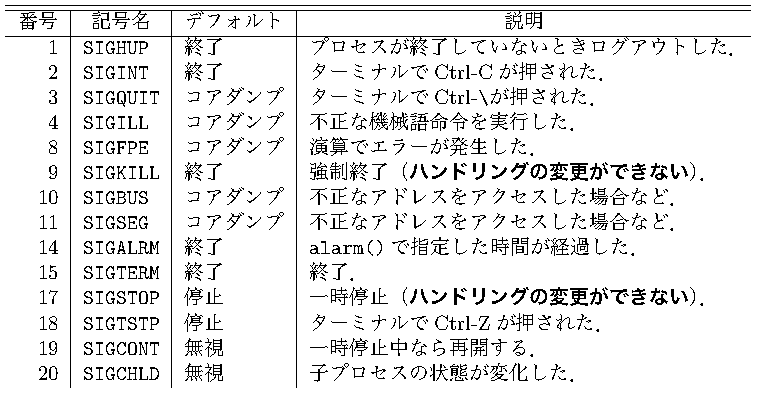
\includegraphics[scale=1.0]{Tbl/signal.pdf}
\end{mytable}

%==============================================================================
\section{シグナルハンドリング}
受け取ったシグナルをプロセスがどのように扱うかを
\emph{シグナルハンドリング}と言う.
シグナルハンドリングは,
次の節で紹介するsignalシステムコールを用いて,
プロセス自身がシグナルの種類ごとに予め決めておく.
指定できるシグナルハンドリングは以下の三種類である.

\begin{enumerate}
\item \emph{無視(ignore)}
  そのシグナルを無視する.

\item \emph{捕捉・キャッチ(catch)}
  そのシグナルを受信し,
  登録しておいたシグナル処理ルーチン(シグナルハンドラ関数)を呼び出す.

\item \emph{デフォルト(default)}
  シグナルの種類ごとに決められている初期のハンドリングであり,
  以下の四種類のどれかである.
  各シグナルのデフォルトが四種類のうちのどれかは\tabref{signal}から分かる.
  %例えばデフォルト状態のまま
  %\texttt{SIGHUP}シグナルを受信するとプロセスは終了するし,
  %\texttt{SIGTSTP}シグナルを受信するとプロセスは停止する.

  \begin{description}
  \item[停止] プロセスは一時停止状態になる.
  \item[無視] プロセスはそのシグナルを無視する.
  \item[終了] プロセスは終了する.
  \item[コアダンプ] プロセスはcoreファイル
    \footnote{プロセスのメモリイメージを書き出したファイルのこと.
      デバッグに使用することができる.
      macOSの標準ではコアダンプしても
      コアファイルを作らないように設定されている.}
    を作成してから終了する.
  \end{description}
\end{enumerate}

%==============================================================================
\section{signalシステムコール}
自プロセスのシグナルハンドリングは signal システムコール\footnote{
  最近のUNIXやmacOSではsignalはライブラリ関数である.
  しかし,古いUNIXではシステムコールだったので,
  ここでは「signalシステムコール」と呼ぶ.}
を使用して変更できる.

\begin{description}
\item[書式] 次の通りである.
\begin{lstlisting}[numbers=none]
  #include <signal.h>
  sig_t signal(int sig, sig_t func);                  // macOSの場合
  __sighandler_t signal(int sig, __sighander_t func); // Ubuntu Linuxの場合
\end{lstlisting}

\item[解説]
  signalシステムコールは,
  自プロセスの指定されたシグナルのハンドリングを変更する.
  \|sig_t|型は関数ポインタ型\footnote{
    関数のアドレスを表す型である.
  }であり,
  \texttt{signal.h}をインクルードすることで自動的に宣言される.

\item[引数]
  第1引数(\texttt{sig})はハンドリングを変更するシグナルの種類である.
  種類は\tabref{signal}に示した番号または記号名で指定する.
  第2引数(\texttt{func})は新しいハンドリングである.
  以下の3種類から一つを指定する.

  \begin{enumerate}
  \item \texttt{SIG\_IGN}はシグナルを無視するようにする.
  \item \texttt{SIG\_DFL}はシグナルハンドリングをデフォルトに戻す.
  \item \emph{シグナルハンドラ関数}を指定する\footnote{
    関数の名前を書けばよい.C言語で関数名は関数を指す関数ポインタになる.}と,
    そのシグナルを捕捉(キャッチ)できるようになる.
    シグナルを捕捉した時にシグナルハンドラ関数が実行される.
    シグナルハンドラ関数の型は\|void func(int sig);|でなければならない.
    引数\texttt{sig}には捕捉したシグナルの番号が渡される.
  \end{enumerate}

\item[戻り値]
  正常なら変更前のハンドリングが返される.
  これを\texttt{sig\_t}型の変数に記録しておけば,
  後でハンドリングをもとに戻すことができる.
  エラーが発生した場合は\texttt{SIG\_ERR}が返され,
  \texttt{errno}変数にエラー番号がセットされる\footnote{
    後で\texttt{perror()}関数が\texttt{errno}変数を参照して,
    エラー原因を表示することができる.}.

\item[プログラム例] signalシステムコールを使用するプログラムの例を二つ示す.
  \begin{enumerate}
  \item \emph{シグナルを無視する例} \\
    リスト\ref{ignore}に\texttt{SIGINT}を一時的に無視するプログラムの例を示す.
    5行でCtrl-Cを無視するようにハンドリングを変更する.
    6行ではCtrl-Cを押してもプログラムが終了しない状態になっている.
    7行でハンドリングを元に戻しCtrl-Cで終了するようにする.

    \lstinputlisting[numbers=left,caption=シグナルを無視する例,
      label=ignore,float=btp]{Lst/signalIgnore.c}
    
  \item \emph{シグナルを捕捉する例} \\
    リスト\ref{catch}に\texttt{SIGINT}を捕捉するプログラムの例を示す.
    9行から11行の間を実行中は,
    Ctrl-Cが押される度に\texttt{handler()}関数が実行される.
  
    \lstinputlisting[numbers=left,caption=シグナルを補足する例,
      float=btp,label=catch]{Lst/signalCatch.c}
  \end{enumerate}

\end{description}

%==============================================================================
\section{シグナルハンドラの制約}
シグナルは割り込みのようなものなので,
ハンドラ関数はいつ呼び出されるか分からない.
そのためシグナルハンドラ中でやって良い処理には強い制約がある.
例えば\texttt{printf()}を実行している途中で
シグナルが発生した場合を考えて欲しい.
シグナルハンドラの内部で\texttt{printf()}関数を呼出したらどうなるだろうか.
何かまずいことが起こりそうな気がする.

\subsection{制約がある理由}
\texttt{printf()}関数を例に制約が必要な理由を考えてみよう.
\texttt{printf()}は高水準I/Oの関数なので出力する内容を一旦バッファに書き込む.
バッファに書き込む処理の最中にシグナルが発生し,
シグナルハンドラが呼出されたとする.

もしも,
シグナルハンドラ中に\texttt{printf()}の呼び出しが含まれていると,
新しい\texttt{printf()}も同じバッファに出力を書き込むので,
バッファのデータが壊れるかもしれない.
\texttt{printf()}に限らず多くのライブラリ関数は,
シグナルハンドラから呼び出されることを前提に設計されていない.

\subsection{やってもよいこと}
\texttt{printf()}関数の例では説明できなかった他の理由もあるので,
シグナルハンドラでは次の三つのことしかやってはならない.

\begin{enumerate}
\item シグナルハンドラ関数のローカル変数の操作
\item \texttt{volatile sig\_atomic\_t} 型変数の読み書き
  \footnote{\texttt{sig\_atomic\_t} 型はmacOSでは\texttt{int}型である.
    \texttt{volatile}を付けるとCコンパイラの最適化の対象外になる
           (詳細はコンパイラにより異なる.).
           コンパイラの最適化は変数がシグナルハンドラなどから非同期に
           アクセスされることを前提にしていない.
           更に注意が必要なことは,これらの制約がある上に「読み書き」が
           単純な\emph{参照}と\emph{代入}のことしか指していないことである
           (インクリメントが正しく動く保証はない.).}
\item 非同期シグナル安全な関数の呼び出し
\end{enumerate}

非同期シグナル安全な関数は,
例えば次のような関数(システムコールも含む)である\footnote{
詳細はオンラインマニュアル\texttt{man 2 sigaction} を参照のこと.}.

\texttt{\_exit(), alarm(), chdir(), chmod(), close(), creat(), dup(),
dup2(), execle(), execve(), fork(), kill(), link(), lseek(), mkdir(),
open(), pause(), read(), rename(), rmdir(), signal(), sleep(), stat(),
time(), unlink(), wait(), write(), strcpy(), strcat(), ...}

%==============================================================================
\section{シグナルハンドラの例}
リスト\ref{handler}に Ctrl-C を三回押すまで終了しないプログラムの例を示す.
3行はシグナルハンドラから操作して良い変数\texttt{flg}を宣言している.
4行からがシグナルハンドラ関数である.
シグナルハンドラは\texttt{flg}の単純な代入と,
非同期シグナル安全な\texttt{write()}の実行しかしない.

\lstinputlisting[numbers=left,caption=シグナルハンドラの例,label=handler,
  float=btp]{Lst/signalHandler.c}

10行で\texttt{handler()}を\texttt{SIGINT}のハンドラ関数として登録している.
11行のwhile文で,変数\texttt{flg}が1になった回数を数えている.
\texttt{main()}でも\texttt{flg}は単純な\emph{参照}と\emph{代入}しかしない.
このように,ハンドラ関数ではフラグを立てることと,
安全なシステムコールの呼び出し程度のことしかできない.

%==============================================================================
\section{killシステムコール}
プロセスがプロセスにシグナルを送信するシステムコールである.

\begin{description}
\item[書式] 以下の通りである.
\begin{lstlisting}[numbers=none]
  #include <signal.h>
  int kill(pid_t pid, int sig);
\end{lstlisting}

\item[解説]
  killシステムコールは,
  送信先のプロセスとシグナルの種類を指定してシグナルを送信する.

\item[引数]
  第1引数(\texttt{pid})は送信先プロセスのプロセス番号である.
  \|pid_t|はプロセス番号を格納するのに都合の良い整数型である.
  第2引数(\texttt{sig})は送信するシグナルの種類である.
  種類は\tabref{signal}に示した記号名または番号で指定する.

\item[戻り値]
  正常時に0,異常時に-1が返される.
  その際,エラー番号が\|errno|変数にセットされる.

\item[プログラム例]
  リスト\ref{kill}にkillシステムコールの使用例として,
  killコマンドを簡単化したプログラム(mykill)を示す.
  このプログラムは,シグナル番号とプロセス番号を引数に実行し,
  指定されたシグナルを指定されたプロセスに送信する.
  11,12行の\|atoi()|関数は,
  10進数を表す文字列(例えば\|"123"|)から整数値(int型の123)を
  求める関数である\footnote{
    詳しくはオンラインマニュアル\texttt{man 3 atoi}で調べること.}.
  リスト\ref{grapher}に,このプログラムの使用例を示す.

\lstinputlisting[numbers=left,caption=簡易killプログラム(mykill),
  float=btp,label=kill]{Lst/mykill.c}

\lstinputlisting[numbers=left,caption=簡易killプログラム(mykill)の実行例,
  label=grapher,numbers=none,float=btp]{Lst/mykill.txt}

\end{description}

%==============================================================================
\section{シグナルと合わせて使うシステムコール}

プロセスを待ち状態にするシステムコール\footnote{
本当はライブラリ関数であるが,
古いUNIXではシステムコールだったので,
ここではシステムコールと呼ぶ.}と,
シグナルを予約するシステムコールを紹介する.

\subsection{sleepシステムコール}
自プロセスを指定された時間,またはシグナルを受信するまで,
待ち状態にする.

\begin{description}
\item[書式] 以下の通りである.

\begin{lstlisting}[numbers=none]
  #include <unistd.h>
  unsigned int sleep(unsigned int seconds);
\end{lstlisting}

\item[解説]
  sleepシステムコールは時間を決めて自プロセスを待ち状態にする.
  もしも待ち状態になっている間にシグナルが届いた場合は,
  そのシグナルのハンドリングが\emph{無視以外}なら,
  待ち状態が解除される(sleepシステムコールが終了する.).
  シグナルを捕捉した場合は直ちにシグナルハンドラが実行される.

\item[引数]
  \texttt{seconds}は待ち時間を秒単位で指定する.

\item[戻り値]
  待ち時間が経過してsleepシステムコールが終了した場合は0が返される.
  シグナルで終了した場合はsleep予定だった残りの秒数が返される.
  
\item[プログラム例]
  リスト\ref{sleep}に1秒に一度\|hello|と表示するプログラムを示す.

  \lstinputlisting[caption=sleepシステムコールの使用例,language=C,
    float=btp,label=sleep]{Lst/sleep.c}

\end{description}

\subsection{pauseシステムコール}
時間制限がないsleepシステムコールである.

\begin{description}
\item[書式] 以下の通りである.

\begin{lstlisting}[numbers=none]
  #include <unistd.h>
  int pause(void);
\end{lstlisting}

\item[解説]
  pauseシステムコールはシグナルが到着するまでプロセスを待ち状態にする.
  シグナルを受信した時の動作はsleepシステムコールと同様である.
  シグナルを受信した時,
  ハンドリングが\emph{終了}になっている場合はプロセスが終了する.
  ハンドリングを\emph{捕捉}にしてから待たなければならない.

\item[戻り値]
  -1が返される.(常時エラー)\footnote{
    シグナルによってエラーが発生しpauseシステムコールが打ち切られた
    という意味である.
  }

\item[プログラム例]
  リスト\ref{pause}は
  シグナルが三回発生するのを pause システムコールで待つプログラムである.
  ハンドリングを捕捉にしていないと一回目のCtrl-Cでプログラムが終了するので,
  何もしないハンドラ関数を登録している.

  \lstinputlisting[caption=pauseシステムコールの使用例,language=C,
    float=btp,label=pause]{Lst/pause.c}

\end{description}

\subsection{alarmシステムコール}
アラームシグナルの発生を予約するシステムコールである.

\begin{description}
\item[書式] 以下の通りである.

\begin{lstlisting}[numbers=none]
  #include <unistd.h>
  unsigned int alarm(unsigned int seconds);
\end{lstlisting}

\item[解説]
  alarmシステムコールは
  \texttt{SIGALRM}シグナルが
  \texttt{seconds}秒後に発生するようにタイマーに予約をする.
  alarmシステムコールは予約するだけで待ち状態になる訳ではない.

\item[引数]
  \texttt{seconds}秒後にシグナルを発生する.
  0 を指定した場合は以前の予約を取り消す.

\item[戻り値]
  通常は0が返される.
  既に別の予約がされていた場合は前の予約の残り時間を返し,
  今回の\texttt{seconds}を用いてタイマーを再起動する.

\item[プログラム例]
  リスト\ref{alarm}は
  アラームシグナルが発生するまで
  pause システムコールで待つプログラムの例である.
  alarm システムコールはシグナルの予約をするだけなので,
  pause システムコールでプログラムを停止する必要がある.

  \lstinputlisting[caption=alarmシステムコールの使用例,language=C,
    float=btp,label=alarm]{Lst/signalAlarm.c}

\end{description}

\section*{課題 No.6}
\begin{enumerate}
\item リスト\ref{handler}のプログラムは,
  Ctrl-Cが押された回数を\texttt{main()}関数側でカウントしている.
  そのため,
  \texttt{main()}関数の処理が忙しくて
  \texttt{flg}変数を頻繁にチェックできない場合に,
  Ctrl-Cの回数を正確にカウントできないかもしれない.
  
  \texttt{main()}関数の力を借りずにCtrl-Cの回数をカウントし,
  三回目のCtrl-Cのとき\texttt{flg}変数を1にするようにプログラムを改良しなさい.
  %\texttt{main()}関数は\texttt{flg}変数が1になったらすぐに終了するようにする.
  シグナルハンドラ中ではグローバル変数のインクリメントはできないものとする.

  \emph{ヒント:} シグナルハンドラ中で\texttt{signal()}を実行してもよい.

\item sleepシステムコールを用いないで,
  指定秒数プログラムを待ち状態にする関数
  \texttt{mysleep(int seconds)}を作りなさい.

\end{enumerate}
 % シグナル
\chapter{環境変数}
この章では,環境変数について学ぶ.
環境変数はシェルが管理する変数である.
変数とはいえC言語の変数とは全く別の仕組みである.
環境変数はシェルから,シェルによって起動されたプロセスにコピーされる.
プロセス(プログラム)は実行時に環境変数の値を調べることができる.
例えば,使用言語を表す環境変数を参照しエラーメッセージの言語を
切り替えるようにプログラムを作っておけば,
一種類のプログラムを世界中で使うことができる.

%==============================================================================
\section{環境変数と使用例}
リスト\ref{environmentVariableSample}に
macOSやUNIXでよく使用される環境変数の「名前」と「値」の例を示す.

\lstinputlisting[numbers=none,caption=よく使用される環境変数,
  label=environmentVariableSample,float=btp]{Lst/environmentVariableSample.txt}

例えば\texttt{LC\_TIME}環境変数は日時の表示に使用する言語を決める.
また,\texttt{TZ}環境変数はどの地域の時刻を表示するか決める.
date コマンド(現在時刻表示),cal コマンド(カレンダー表示),
ls コマンド(ファイルの最終変更時刻表示)等がこれらの環境変数の値により
日時の表示を変化させる.

リスト\ref{environmentVariableLCTIME}に,
これら環境変数の値を変化しながらコマンドを実行した例を示す.
例えばdateコマンドは現在時刻を,
\texttt{LC\_TIME}環境変数の値が\texttt{C}なら英語表記で表示するが,
\texttt{ja\_JP.UTF-8}なら日本語表記で表示する.
\texttt{TZ}環境変数の値が\texttt{Japan}なら日本時間で表示するが,
\texttt{Cuba}ならキューバ時間で表示する.
このように環境変数はプログラムの振る舞いに影響を与える.

\lstinputlisting[numbers=none,caption=環境変数の変化が与える影響の例,
  float=btp,label=environmentVariableLCTIME]{Lst/environmentVariableLCTIME.txt}

%==============================================================================
\section{環境変数を誰が決めるか}

\begin{enumerate}
\item システム管理者 \\
  システム管理者はユーザがログインした時の初期状態を決める.
  UNIXやmacOSでは,\|/etc/profile|ファイル等に書かれたスクリプトが
  全ユーザのシェル起動時に実行される.
  システム管理者は全ユーザに共通のシェルの初期化処理をここに書いておく.
  このスクリプトで全ユーザに共通の環境変数の初期化ができる.
\item ユーザの設定ファイル \\
  ユーザは自分のホームディレクトリの\|.bash_profile|ファイルに
  自分専用の初期化処理を書くことができる.
  ここに,\ref{environmentVariableOperation}で説明するコマンドを
  用いてスクリプトを書いておく.
  以下に\|.bash_profile|ファイルの例を示す\footnote{
    代入(\texttt{=})の左右に空白を書いてはならない.
    以降の書式や実行例でも同様である.}.
  \lstinputlisting[numbers=none]{Lst/dotBashRc.txt}
\item ユーザによるコマンド操作 \\
  シェルのコマンド操作で環境変数を操作することができる.
  但し,影響範囲は操作したウインドのシェルのみである.
  また,次回のログイン時には操作結果の影響は残らない.
\end{enumerate}

%==============================================================================
\section{環境変数の操作}\label{environmentVariableOperation}
以下では,コマンドラインで環境変数を操作する方法を解説する.

\subsection{表示}
printenv コマンドを用いて環境変数を表示する.

\begin{description}
\item[書式] \texttt{name}は環境変数の名前である.
\begin{lstlisting}[numbers=none]
  printenv [name]
\end{lstlisting}
\item[解説]
  \texttt{name} を省略した場合は,
  全ての環境変数の名前と値を表示する.
  \texttt{name} を書いた場合は該当のする環境変数の\emph{値だけ}表示する.
  該当する環境変数が無い場合は何も表示しない.
\item [実行例]  macOS 上での printenvコマンドの実行例を示す.
  環境変数の名前を省略して実行した場合は,
  全ての環境変数について「名前=値」形式で表示される.
  \lstinputlisting[numbers=none]{Lst/environmentVariablePrintenv.txt}
\end{description}

\subsection{新規作成(その1)}
UNIXの標準シェル(sh)での操作方法を説明する.

\begin{description}
\item[書式] 次の2ステップで操作を行う.
\begin{lstlisting}
  name=value
  export name
\end{lstlisting}
\item[解説]
  1行で,一旦,シェル変数を作る.
  2行でシェル変数を環境変数に変更する.
\item[実行例]
  1行は\texttt{MYNAME}環境変数が存在するか確認している.
  \texttt{MYNAME}環境変数は存在しないので何も表示されない.
  2,3行で値が\texttt{sigemura}の\texttt{MYNAME}環境変数を作った.
  4行で\texttt{MYNAME}環境変数を確認すると
  値が\texttt{sigemura}になっていることが分かる.
  \lstinputlisting[numbers=left]{Lst/environmentVariableSh.txt}
\end{description}

\subsection{新規作成(その2)}
macOSやLinuxで使用されるシェル(bash)では,
次のように1行の操作で環境変数を作ることができる.

\begin{description}
\item[書式]
  次の1ステップで環境変数を作ることができる.
\begin{lstlisting}[numbers=none]
  export name=value
\end{lstlisting}
\item[解説]
  一旦,シェル変数を作ることなく環境変数を作ることができる.
\item[実行例]
  次のように動作確認ができる.
  \lstinputlisting[numbers=none]{Lst/environmentVariableBash.txt}
\end{description}

\subsection{値の変更}
既に存在する環境変数の値を変更することができる.

\begin{description}
\item [書式]
  \texttt{name}は環境変数の名前,\texttt{value}は新しい値である.
\begin{lstlisting}[numbers=none]
  name=value
\end{lstlisting}
\item [解説]
  「環境変数の変更」と「シェル変数の作成」は書式だけでは区別が付かない.
  変数名を間違った場合,
  間違った名前で新しいシェル変数が作成されエラーにならないので
  注意が必要である.
\item [実行例]
  \texttt{MYNAME}環境変数が既に存在している場合の実行例を示す.
  \lstinputlisting[numbers=none]{Lst/environmentVariableOverWrite.txt}
\end{description}

\subsection{値の参照}
環境変数やシェル変数の値を利用することができる.

\begin{description}
\item [書式]
  \texttt{name}は環境変数の名前である.
\begin{lstlisting}[numbers=none]
  $name
\end{lstlisting} %$
\item [解説]
  \texttt{\$name}は,
  シェルが入力されたコマンドの意味を評価する際に,
  変数の値に置き換えられる.
\item [実行例1]
  すでにある\texttt{PATH}環境変数の値に新規ディレクトリを追加する\footnote{
    システムが決めたディレクトリに,
    ユーザがディレクトリを追加することはよくある.
  }例を示す.
  \lstinputlisting[numbers=none]{Lst/environmentVariableReference.txt}
\item [実行例2]
  環境変数\texttt{i}の値を数値と見做してインクリメント\footnote{
    \texttt{expr}コマンドとsh(bash)のコマンド置換を使用している.
  }する例を示す.
  \texttt{printenv i}の代わりに\texttt{echo \$i}でも値を表示できる.
  \lstinputlisting[numbers=none]{Lst/environmentVariableIncrement.txt}
\end{description}

\subsection{変数の削除}
unsetコマンドを用いて,
環境変数やシェル変数を削除することができる.

\begin{description}
\item [書式]
  \texttt{name}は変数の名前である.
\begin{lstlisting}[numbers=none]
  unset name
\end{lstlisting}
\item [解説]
  存在しない変数を\texttt{unset}してもエラーにならない.
  変数名を間違ってもエラーにならないので注意が必要である.
\item [実行例]
  \texttt{MYNAME}環境変数が既に存在している場合の実行例を示す.
  \lstinputlisting[numbers=none]{Lst/environmentVariableUnset.txt}
\end{description}

\subsection{一時的な作成と値の変更}
env コマンドを用いて,
環境変数の値を一時的(今回のコマンド実行の期間だけ)に
変更してコマンド(プログラム)を実行したり,
一時的に環境変数を作ってコマンドを実行したりすることができる.

\begin{description}
\item [書式]
  変数へ値を代入する指示が続いた後に,実行するコマンドが続く.
\begin{lstlisting}[numbers=none]
  env name1=value1 name2=value2 ... command
\end{lstlisting}
\item [解説]
  env コマンドは代入形式のコマンド行引数が続く間,
  それらを環境変数の変更(作成)指示とみなし処理する.
  代入形式ではないコマンド行引数を見つけたら,
  それ以降を実行すべきコマンドとみなす.
\item [実行例]
  ロケール\footnote{
    囲み記事「ロケール」を参照のこと.
  }とタイムゾーン\footnote{
    囲み記事「タイムゾーン」を参照のこと.
  }を変更してdateコマンドを実行する例である.
  日時表示用のロケールを格納する\texttt{LC\_TIME}変数を日本語表示を示す値に,
  タイムゾーンを格納する\texttt{TZ}変数をキューバ時間を表す値に変更した上で,
  dateコマンドを実行している.
  その後でdateコマンドをもう一度実行し,
  環境変数の変更が一時的であることを確認している.
  \lstinputlisting[numbers=none]{Lst/environmentVariableEnv.txt}
\end{description}

\begin{figure}[btp]
\begin{itembox}[l]{ロケール}
\texttt{LANG}環境変数や\texttt{LC\_TIME}環境変数に
セットする値をロケール名と呼ぶ.
ロケール名は「言語コード」,「国名コード」と「エンコーディング」の
組み合わせで表現される.

\begin{itemize}
\item
  言語コード\footnote{
  言語コードは\url{https://ja.wikipedia.org/wiki/ISO_639-1}等を参照のこと.
  }はISO639で定義された2文字コードである(日本語は"ja").
\item 
  国名コード\footnote{
    国名コードは\url{https://ja.wikipedia.org/wiki/ISO_3166-1}等を参照のこと.
  }はISO3166で定義された2文字コードである(日本は"JP").
\item
  エンコーディングは,使用する文字符号化方式を示す.
  エンコーディングがターミナルエミュレータの
  テキストエンコーディングと一致していないと文字化けを起こす
  (macOSではUTF-8方式が使用される.).
\end{itemize}

使用可能なロケールの一覧は\|locale -a|コマンドで表示できる.
通常,macOSで日本語を使用する場合のロケール名は,
言語コード=\texttt{ja},国名コード=\texttt{JP},エンコーディング=\texttt{UTF-8}を
組み合わせて次のようになる.

\centerline{\texttt{ja\_JP.UTF-8 }(日本語\_日本.UTF-8)}
\end{itembox}
\end{figure}

\begin{figure}[btp]
\begin{itembox}[l]{タイムゾーン}
\texttt{TZ}環境変数にタイムゾーンを表す値をセットする.
macOSやUNIXの内部で時刻は協定世界時(UTC)で管理されており,
時刻を表示する時に現地時間に変換して表示する.
時刻に関係するプログラムは
協定世界時と現地時間の変換方法を\texttt{TZ}環境変数から知ることができる.
日本の場合はタイムゾーン名が\texttt{JST},協定世界時との時差が$-9$時間なので,
\|TZ=JST-9|となる.

この形式の他に\|/usr/share/zoneinfo/|に置いてあるファイル名で
タイムゾーンを指定することもできる.
\|/usr/share/zoneinfo/Cuba|ファイルが存在するので
\|TZ=Cuba|と指定できる.
\|/usr/share/zoneinfo/Japan|ファイルも存在するので
\|TZ=Japan|も指定できる.
\|/usr/share/zoneinfo/Asia/Tokyo|ファイルが存在するので
\|TZ=Asia/Tokyo|と指定しても良い.

なお,\texttt{TZ}環境変数が定義されていない時は,
OSのインストール時に選択した標準のタイムゾーンが用いられる.
\end{itembox}
\end{figure}

\newpage
空のページ
\newpage
%==============================================================================
\section{環境変数の仕組み}
環境変数を管理する仕組みと,
環境変数をプロセス間で引き継ぐ仕組みを学ぶ.

\subsection{シェルによる管理}
シェルもプログラムの一種なので,
\figref{proc}に示したようなプロセスとして実行される.
\figref{environmentVariableShell}は,
\figref{proc}をシェルプロセスの場合に当てはめた図である.
シェルプロセス(shellプロセス)は
環境変数を自プロセスのデータ領域に\footnote{
本当はスタック領域も使っているかも知れない.}記憶している.
ユーザが\|export|や\|unset|等のコマンドを入力すると,
シェルプログラムのインタプリタが意味を解釈し環境変数を操作する.
なお,これらのシェル自身が処理するコマンドを\emph{内部コマンド}と呼ぶ.

\begin{myfig}{btp}{環境変数をシェルの内部で管理}{environmentVariableShell}
  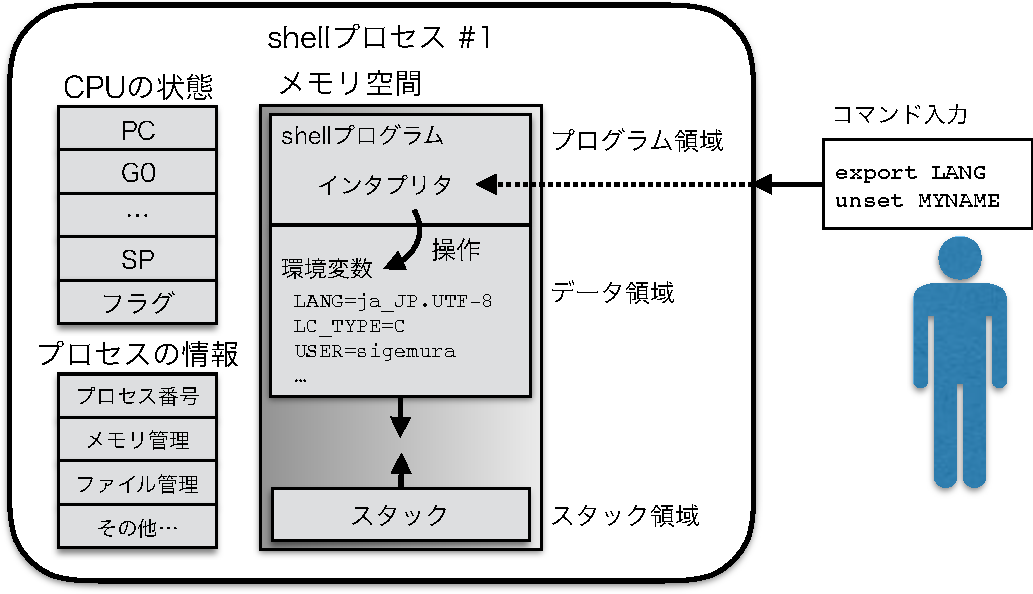
\includegraphics[scale=0.70]{Fig/environmentVariableShell-crop.pdf}
\end{myfig}

\subsection{プロセスへのコピー}
\figref{environmentVariableCopy}に示すように,
シェルは入力されたコマンドが内部コマンド以外(\emph{外部コマンド})なら,
コマンド名と同じ名前のプログラムを探し子プロセスとして起動する.
この時シェルは,
自身の環境変数を子プロセスにコピーするようにOSカーネルに依頼する.
OSカーネルは子プロセスのメモリ空間のどこか(例えばスタックの底)に
環境変数をコピーする.
子プロセスは,
自身のメモリ空間にコピーされた環境変数を,
参照・変更・削除できる.

\begin{myfig}{btp}{プログラム起動時の環境変数コピー}{environmentVariableCopy}
  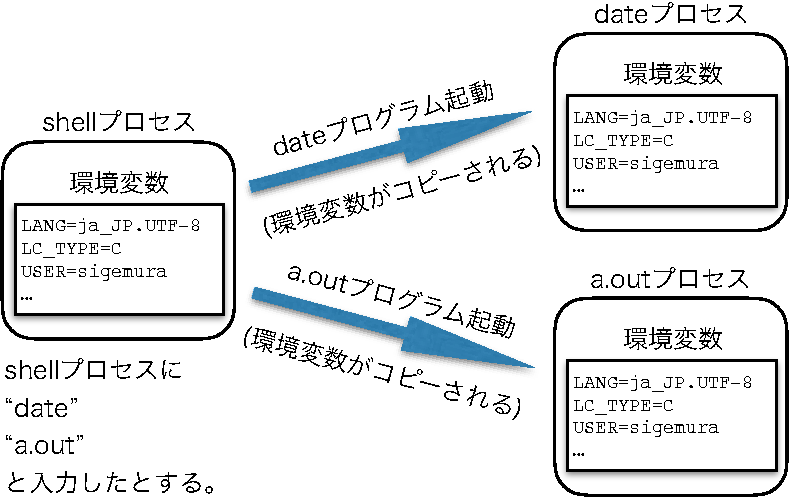
\includegraphics[scale=0.75]{Fig/environmentVariableCopy-crop.pdf}
\end{myfig}

\subsection{変更した上でのコピー}
プロセスへ環境変数をコピーする仕組みは,
シェルに限らず全ての他のプログラムを起動するプログラムで共通に用いられる.
\ref{environmentVariableOperation}で紹介したenvコマンドも,
この仕組を利用している.

envコマンドは\emph{外部コマンド}である.
envコマンドは他のプログラムを起動するプログラムとして実装できる.
\figref{environmentVariableEnv}にenvコマンドの仕組みを示す.
envコマンドは自身の環境変数を変更した後,
目的のプログラムを起動する.
その時,新しいプログラムに変更後の環境変数がコピーされる.

\begin{myfig}{btp}{env プログラムの仕組み}{environmentVariableEnv}
  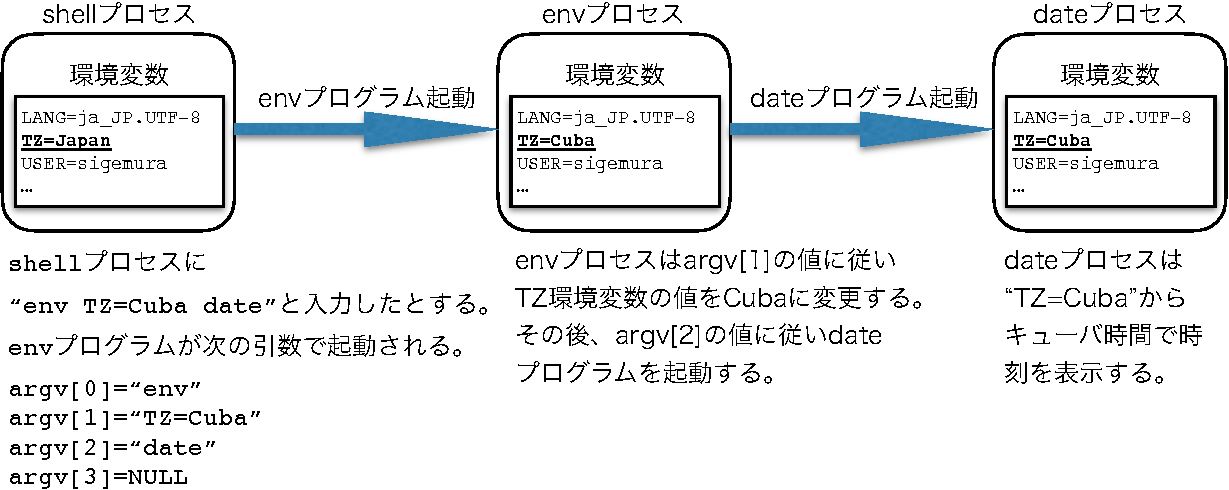
\includegraphics[scale=0.8]{Fig/environmentVariableEnv-crop.pdf}
\end{myfig}

%==============================================================================
\section{プログラムからの環境変数アクセス}
C言語プログラムから環境変数をアクセスする方法を紹介する.

\subsection{読み出し}
C言語から環境変数を読み出すために,
以下に紹介する二つの方法が使用できる.

\begin{enumerate}
\item \emph{\texttt{main}関数の\texttt{envp}仮引数や
  グローバル変数\texttt{environ}を用いる.} \\
  C言語の\|main()|関数には,実は第三引数\|envp|が存在している.
  また,\|environ|という名前のC言語のグローバル変数も存在する.
% これらは\figref{environmentVariableData}のように初期化されているので,
  これらから環境変数のリストを読み出すことができる.

  \begin{description}
  \item [書式]
    \|environ|変数はライブラリのどこかで定義されいて,
    C言語プログラムからは1行目のように宣言すれば参照できるようになる.
    \|main()|の第三引数まで含めたプロトタイプ宣言は2行目の通りである.

\begin{lstlisting}[numbers=left]
extern char **environ;
int main(int argc, char *argv[], char *envp[]);
\end{lstlisting}

  \item [解説]
    \|environ|変数と\|main()|関数の\|envp|引数は,
    \figref{environmentVariableData}のように初期化される.
    例えば全ての環境変数を表示するCプログラムは
    次のように書くことができる.
    まず,2行目のように書くことで\|environ|変数を参照可能になる.
    \|environ|変数は文字列を指すポインタの配列を指しているので,
    \|environ[i]|の記述は\|LANG=ja_JP.UTF-8|等の文字列を意味する.
    配列の末尾には\|NULL|ポインタが格納されているので,
    これを目印にループを終了する(4行).
    %リスト\ref{environmentVariablePrintAll}のように書くことができる.

    \begin{myfig}{btp}{環境変数のデータ構造}{environmentVariableData}
      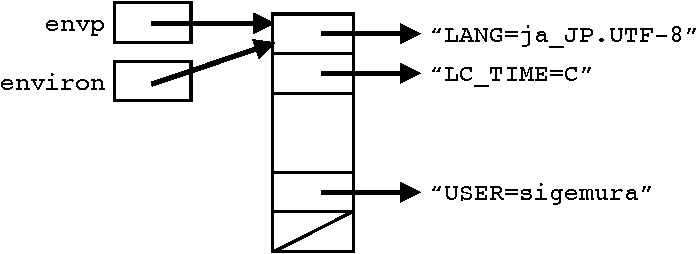
\includegraphics[scale=0.8]{Fig/environmentVariableData-crop.pdf}
    \end{myfig}

    \lstinputlisting[numbers=left
      %,caption=全ての環境変数を印刷するプログラム
      %,label=environmentVariablePrintAll
    ]{Lst/environmentVariablePrintAll.c}
  \end{description}

\item \emph{\texttt{getenv}関数を用いる.} \\
  \|getenv()|ライブラリ関数を用いて
  名前で指定した環境変数の値を読み出すことができる.

  \begin{description}
  \item [書式] \|getenv()|は次のような書式の関数である.

\begin{lstlisting}[numbers=none]
#include <stdlib.h>
char *getenv(char *name);
\end{lstlisting}

  \item [解説] \|name|には環境変数名を渡す.
    \|getenv()|は環境変数の値を表す文字列を指すポインタを返す.
    \|name|の環境変数が見つからない場合は\|NULL|ポインタを返す.

  \item [プログラム例]
    %リスト\ref{environmentVariablePrintLANG}のCプログラムは
    次のCプログラムは
    \|LANG|環境変数の値を表示するものである.
    4行で\|LANG|環境変数を探し,それの値(文字列)を指すポインタを返す.
    \|LANG|環境変数が見つかったら6行で\|LANG=|に続けて値を表示する
    (表示例は14行).
    見つからない場合は8行で見つからなかったことを意味するメッセージを表示する.

    \lstinputlisting[numbers=left
      %,caption=LANG環境変数の値を表示するプログラム,
      %,label=environmentVariablePrintLANG
    ]{Lst/environmentVariablePrintLANG.c}
  \end{description}
\end{enumerate}

\subsection{操作}
自プロセスのメモリ空間にコピーされた環境変数を操作する
三つのC言語ライブラリ関数を紹介する.
なお,一旦,環境変数を追加・変更・削除する操作を行うと
\|main()|の仮引数\|envp|は使用できなくなる(値がデタラメになる).
常にグローバル変数\|environ|を使用するとトラブルが少ない.

\begin{enumerate}
\item \emph{\texttt{setenv}関数} \\
  環境変数を新規に作成したり,値を上書きしたりする関数である.

  \begin{description}
  \item [書式] \|setenv()|は次のような書式の関数である.

\begin{lstlisting}[numbers=none]
#include <stdlib.h>
int setenv(char *name, char *val, int overwrite);
\end{lstlisting}

  \item [解説]
    \|name|は環境変数の名前,
    \|val|は環境変数にセットする値である.
    \|overwrite|は,\|0|の時に上書き禁止,
    それ以外の時に上書き許可を意味する.
    \|setenv()|は正常時に\|0|,エラー時に\|-1|を返す.
    上書き禁止の時,既に同じ名前の環境変数が存在するとエラーになる.
    エラー時は\|errno|大域変数にエラー番号がセットされる.

  \item [使用例] \|MYNAME|環境変数の値を\|sigemura|にする例を示す.
    第3引数が\|1|なので,
    \|MYNAME|環境変数が既に存在する場合は値の上書きになり,
    エラーにはならない.

\begin{lstlisting}[numbers=none]
setenv("MYNAME", "sigemura", 1);
\end{lstlisting}
  \end{description}

\item \emph{\texttt{putenv}関数} \\
  環境変数を新規に作成したり,値を上書きしたりする関数である.

  \begin{description}
  \item [書式] \|putenv()|は引数を一つだけ持つ.

\begin{lstlisting}[numbers=none]
#include <stdlib.h>
int putenv(char *string);
\end{lstlisting}

  \item [解説]
    \|string|は\|NAME=VALUE|形式の文字列である
    (それ以外の形式の文字列を渡すとエラーになる).
    \|putenv()|は正常時に\|0|,エラー時に\|-1|を返す.
    エラー時は\|errno|大域変数にエラー番号がセットされる.
    \|putenv("NAME=VALUE");|は,
    \|setenv("NAME","VALUE",1);|と同じ操作を行う.

  \item [使用例]
    前出の\|setenv()|の使用例と同じことを\|putenv()|を用いて行う例を示す.

\begin{lstlisting}[numbers=none]
putenv("MYNAME=sigemura");
\end{lstlisting}

  \end{description}

\item \emph{\texttt{unsetenv}関数} \\
  環境変数を削除する関数である.

  \begin{description}
  \item [書式]  \|unsetenv()|も引数を一つだけ持つ.

\begin{lstlisting}[numbers=none]
#include <stdlib.h>
int unsetenv(char *name);
\end{lstlisting}

  \item [解説] \|name|は削除する環境変数の名前である.
    \|unsetenv()|は正常時に\|0|,エラー時に\|-1|を返す.
    エラー時は\|errno|大域変数にエラー番号がセットされる.

  \item [使用例] \|MYNAME|環境変数を削除する例を示す.

\begin{lstlisting}[numbers=none]
unsetenv("MYNAME");
\end{lstlisting}

  \end{description}
\end{enumerate}


%==============================================================================
%\section*{課題 No.7}
%\begin{enumerate}
%\item ここまでの実行例を試してみなさい.
%\item 囲み記事を参考に,
%  \texttt{LC\_TIME}環境変数や\texttt{TZ}環境変数を変更し,
%  効果を確認する.
%  例えば,
%  「モスクワ時間,ロシア語表記」で現在時刻を表示するにはどうしたらよいか?
%\end{enumerate}

%==============================================================================
\section*{課題 No.8}
\begin{enumerate}
\item 外部コマンドprintenvの仕様を調べる \\
  オンラインマニュアル(\|man 1 printenv|)を読んだり,
  \|printenv|を実際に実行したりして,
  printenvコマンドの仕様を調べなさい.
\item myprintenvプログラム\\
  外部コマンドprintenvと同様な働きをするmyprintenvプログラムを作成しなさい.
  なるべく本物と同じ動作をするように作ること.
\end{enumerate}
 
 % 環境変数
\chapter{プロセスの生成とプログラムの実行}
この章では新しいプロセスでプログラムを実行させる方法を学ぶ.
プログラムを起動する方式には大きく分けて,
\emph{spawn方式}(スポーン:卵を産む方式)と,
\emph{fork-exec方式}(分岐-実行方式)がある.

\section{spawn 方式}
Windows等で使用される方式である.
新しい「(1) プロセスを作り」,「(2) プロセスを初期化し」,
「(3) プログラムを実行する」の三つの仕事を一つのspawnシステムコールで行う.
fork-exec方式を実現するためには,
メモリ再配置のためのハードウェア機構を持っている必要がある.
そのため組込用の小さなコンピュータではspawn方式しか選択肢がない場合がある.

UNIX系OSでもspawn方式を使用できる.
次にmacOSの\|posix_spawn|システムコールを紹介する.
新しいプロセスの初期化を指示するデータ構造を渡すようになっている.

\begin{description}
\item[書式] 次の通りである.
\begin{lstlisting}[numbers=none]
  #include <spawn.h>
  int posix_spawn(pid_t *pid, char *path,
                  posix_spawn_file_actions_t *file_actions,
                  posix_spawnattr_t *attrp,
                  char *argv[], char *envp[]);
\end{lstlisting}

\item[解説]
  新しいプロセスを作り\|path|で指定したプログラムを実行する.

\item[引数]
  \|pid|は新しいプロセスのプロセス番号を格納する変数を指すポインタ.
  \|path|は実行するプログラムを格納したファイルのパスである.
  絶対パスでも相対パスでも良い.
  \|file_actions|,\|attrp|はプロセスの初期化を指示するデータ構造へのポインタ.
  \|argv|,\|envp|は実行されるプログラムに渡すコマンド行引数と環境変数である.
\end{description}

\section{fork-exec 方式}
UNIX系のOS用いられてきた方式のことである.
以下に示す次の三つのステップで新しいプログラムを実行する.
また,その様子を\figref{forkExec}に模式的に示す.
\begin{enumerate}
\item 親プロセスが
  新しいプロセス(子プロセス)を作る(\emph{forkシステムコール}).
\item ユーザが記述したプログラムに従い子プロセスが自ら初期化処理を行う.
\item 子プロセスが
  新しいプログラムをロード・実行(\emph{execveシステムコール})する.
\end{enumerate}
この方式はユーザが記述したプログラムで初期化処理を行うので柔軟性が高い.
以下では,fork-exec方式について具体的なプログラム例を示しながら詳しく解説する.

\myfigure{btp}{scale=0.66}{Fig/forkExec-crop.pdf}{fork-exec方式}{forkExec}

\subsection{プログラムのロードと実行(execveシステムコール)}
まず,プロセスが新しいプログラムの実行を開始する
ために使用するexecveシステムコールを紹介する.
\figref{forkExec}では,
作ったばかりの子プロセスにexecveを実行させているが,
普通のプロセスがexecveシステムコールを使用しても良い.
forkと組み合わせて使用する例は後の方で説明することとし,
ここではexecveシステムコール単独で使用する例を示す.

\figref{execve}に execve システムコールを実行するプロセスの様子を示す.
プロセスが execve システムコールを実行すると,
そのプロセスのメモリ空間に新しいプログラムがロードされる.
execve システムコールを実行したプログラムは,
新しいプログラムで上書きされ消えてしまう.
プロセスの仮想CPUはリセットされ,
新しいプログラムが最初から実行される.
プロセスは新しいプログラムを実行するように\emph{変身}した(変身の術).
以下に,UNIXのexecveシステムコールの解説を示す.

\myfigure{btp}{scale=0.8}{Fig/execve-crop.pdf}
         {execveシステムコールの仕組み}{execve}

\begin{description}
\item[書式] execveシステムコールの書式は次の通りである.
\begin{lstlisting}[numbers=none]
  #include <unistd.h>
  int execve(char *path, char *argv[], char *envp[]);
\end{lstlisting}

\item[解説]
  自プロセスで\|path|で指定したプログラムを実行する.
  正常時にはexecveを実行したプログラムは新しいプログラムで上書きされ消える.
  execveシステムコールが戻る(次の行が実行される)のはエラー発生時だけである.

\item[引数]
  \|path|は実行するプログラムを格納したファイルのパスである.
  絶対パスでも相対パスでも良い.
  \|argv|,\|envp|は新しいプログラムに渡すコマンド行引数と環境変数である.

\item[使用例1]
  リスト\ref{exectest1}に execve システムコールを用いて,
  \|/bin/date|プログラムを実行するプログラムの例を示す.
  3行は自身の環境変数を指すポインタ\|environ|を宣言している.
  4行でdateプログラムの\|argv|に渡す配列\|args|を準備した.
  7行のexecveシステムコールで\|/bin/date|プログラムをロード・実行する.
  \|args|,\|environ|は,
  dateプログラムのmain関数の\|argv|と\|envp|に渡される.
  \|environ|を渡したので,
  dateプログラムはこのプログラムと同じ環境変数で実行される.

  execveシステムコールが正常に実行された場合は,
  システムコールを発行したプログラムがdateプログラムによって
  上書きされ消えるので8行以降は実行されない.
  8行が実行されるのはシステムコールの実行に失敗した場合だけである.
  そこでエラー判定(if文)なしにエラー処理(perrorの実行など)を行ってよい.

  \lstinputlisting[label=exectest1
    ,caption=execveの使用例(その1)
    ,float=btp, numbers=left]{Lst/exectest1.c}

\item[使用例2]
  リスト\ref{exectest3}は,
  環境変数の一部を書き換えた上で,
  \|/bin/date|プログラムを実行するプログラムの例である.
  これは,プログラムを実行する前に行う\emph{初期化処理}の例でもある.
  まず8行で初期化処理として\|putenv()|関数を用いて自身の環境変数を書換える.
  execveシステムコールに渡される\|environ|は書換え後のものである.
  \|LC_TIME|環境変数を\|ja_JP.UTF-8|に書換えてあるので,
  15行のように現在時刻が日本語で表示さる.

  \lstinputlisting[label=exectest3
    ,caption=execveの使用例(その2)
    ,float=btp, numbers=left]{Lst/exectest3.c}

\item[使用例3]
  リスト\ref{exectest2}は,
  全く新しい環境変数の一覧を渡して
  \|/bin/date|プログラムを実行する例である.
  4行で\|environ|と同じデータ構造の\|envs|配列を作って,
  7行でexecveシステムコールに渡した.
  \|envs|配列に\|LC_TIME|,\|TZ|環境変数が格納されているので,
  これらが\|/bin/date|プログラムにコピーされる.
  他の環境変数を\|/bin/date|プログラムは必要としていないので,
  13行のように言語とタイムゾーンを変更して正常に動作する.

  \lstinputlisting[label=exectest2
    ,caption=execveの使用例(その3)
    ,float=btp, numbers=left]{Lst/exectest2.c}

\item[使用例4]
  リスト\ref{exectest4}は,
  複数のコマンド行引数がある場合の例である.
  \|/bin/echo|プログラムを \|aaa|, \|bbb| を引数にして実行する.
  \|args|配列にプログラムの名前(\|argv[0]|のための\|"echo"|)を
  忘れないように注意すること.

  \lstinputlisting[label=exectest4
    ,caption=execveの使用例(その4)
    ,float=btp, numbers=left]{Lst/exectest4.c}

\end{description}

\subsection{execveシステムコールのラッパー関数}
execveシステムコールを使いやすくするライブラリ関数を紹介する.
ここで紹介する関数は内部でexecveシステムコールを呼び出す.
これらの関数はexecveシステムコールの
\emph{ラッパー(wrapper)関数}になっている.

\begin{description}
\item[書式]
  execve システムコールの四つのラッパー関数の書式をまとめて掲載する.
\begin{lstlisting}[numbers=none]
  #include <unistd.h>
  int execv(char *path, char *argv[]);
  int execvp(char *file,  char *argv[]);
  int execl(char *path, char *argv0, *argv1, ... ,*argvn, NULL);
  int execlp(char *file, char *argv0, *argv1, ... ,*argvn, NULL);
\end{lstlisting}

\item [解説]
  \emph{\texttt{execv()}関数}は環境変数を指定する必要がないexec関数である.
  常に自プログラムの環境変数\|environ|をexecveシステムコールに渡す.
  execveシステムコールとの関係は次のようになる.

  \centerline{\texttt{execv("/bin/date", argv);}
    →  \texttt{execve("/bin/date", argv, environ);}}

  \emph{\texttt{execvp()}関数}は,\|execv()|関数にPATH環境変数を用いた
  プログラムファイルの検索機能を追加したものである.
  第一引数に\|/bin/date|のようなパスではなく\|date|のような
  ファイル名だけ渡すと,自動的にPATH環境変数を使用した検索を行い
  \|/bin/date|プログラムを発見して実行してくれる.
  
  \centerline{\texttt{execvp("date", argv);}
    →  \texttt{execve("/bin/date", argv, environ);}}

  \emph{\texttt{execl()}関}数は,\|execv()|関数の\|argv|配列の代わりに
  複数の文字列を渡すことができる関数である.
  文字列の個数は可変なので終わりを示す\| NULL|を最後に置く必要がある.
  リスト\ref{exectest4}のexecveシステムコールを次のように書換えることで,
  同じ結果を得ることができる.
  \|argv[0]|に渡す\|"echo"|を忘れないように注意が必要である.

  \centerline{\texttt{execl("/bin/echo", "echo", "aaa", "bbb", NULL);}}

  \emph{\texttt{execlp()}関数}は,\|execl()|関数にPATH環境変数を用いた
  プログラムファイルの検索機能を追加したものである.

  \centerline{\texttt{execlp("echo", "echo", "aaa", "bbb", NULL);}}

\end{description}

\subsection{入出力のリダイレクト}
execveする際,プロセス状態(\figref{execve}参照)の一部が引き継がれる.
例えば,PID(プロセス番号),
オープン中のファイルや入出力,
カレントディレクトリ,
「無視」に設定されたシグナルハンドリング等は,
新しいプログラムに引き継がれる.
プログラムが最初から標準入力(0),標準出力(1),
標準エラー出力(2)を利用できるのは,
execve前にオープンされていた入出力を引き継ぐからである..

シェルがプログラムを実行する際は,
シェルは標準入力をキーボード用にオープンし,
標準出力と標準エラー出力をディスプレイ用にオープンした状態
\footnote{
  既にシェル自身用にオープン状態になっているので,
  わざわざ,オープンし直す必要は無い.}
で目的のプログラムをexecveする.
シェルのリダイレクト(プログラムの入出力を切替える仕組み)は,
リダイレクト先のファイルを標準入力・出力としてオープンした状態で
目的のプログラムをexecveすることで実現している.

\lstinputlisting[label=exectest5
  ,caption=標準出力をリダイレクトして\texttt{/bin/echo}を実行する例
  ,float=btp, numbers=left]{Lst/exectest5.c}

リスト\ref{exectest5}は,
標準出力を\|aaa.txt|ファイルにリダイレクトした状態で
\|/bin/echo|を実行するプログラムである.
まず,初期化処理(\figref{forkExec}参照)として
7行と8行で標準出力のリダイレクトを行っている.
7行の\|close(1)|は標準出力(ファイルディスクリプタ1番)をクローズする.
8行の\|open()|はファイルディスクリプタ番号を小さい順に使用するので,
\|close(1)|直後の\|open()|は1番のファイルディスクリプタを返す.
ここまでで,
標準出力である1番のファイルディスクリプタがファイルにリダイレクトされた.
次に,14行のexecveシステムコールで自身がechoプログラムに変身する.

\subsection{新しいプロセスを作る(forkシステムコール)}
execveシステムコールはプロセスを新しいプログラムに変身させる.
変身して新しいプログラムを実行したプロセスは終了してしまう.
プロセスの数は減る一方である.
新しいプロセスを作って,新しいプログラムを実行させる仕組みが必要である.
forkシステムコールは新しいプロセスを作成し自身をコピーする.
つまり,\emph{分身}を作るシステムコールである(分身の術).
次にUNIXのforkシステムコールを説明する.

\begin{description}
\item[書式] fork の書式を示す.
\begin{lstlisting}[numbers=none]
  #include <unistd.h>
  int fork(void);
\end{lstlisting}

\item[解説] forkシステムコールを実行した瞬間の,プロセスのコピーを作る.
  元のプロセスを\emph{親プロセス},
  コピーして作ったプロセスを\emph{子プロセス}と呼ぶ.
  \figref{fork}に模式図を示す.
  親プロセスと子プロセスではPID(プロセス番号)を除き全く同じになる.
  CPUの状態もコピーされるので,
  子プロセスはforkシステムコールの途中から実行が開始される.

  \myfigure{btp}{scale=0.8}{Fig/fork-crop.pdf}{forkの仕組み}{fork}

  forkシステムコールが終了する際,
  親プロセスには子プロセスのPIDが返され,
  子プロセスには\|0|が返される.
  プログラムはこの値を目印に自分が親か子か判断できる.
  エラー時は,親プロセスに\|-1|が返され子プロセスは作られない.

\item[使用例]
  リスト\ref{forktest}にforkシステムコールを実行するプログラムの例を,
  以下にforkの処理手順を示す.
  最終的に親プロセスと子プロセスが同時に並行して実行される状態になる.

  \lstinputlisting[label=forktest
    ,caption=forkシステムコールの使用例
    ,float=btp, numbers=left]{Lst/forktest.c}
  
  \begin{enumerate}
  \item 6行で親プロセスがforkシステムコールを実行する.
    \figref{fork}のように,
    新しいプロセス(子プロセス)が作られ,親プロセスの内容がコピーされる.
    子プロセスには,
    メモリ空間(プログラム,変数(データ),スタック),
    プロセスの状態(どのファイルをオープン中か,シグナルハンドラの登録等),
    CPUの状態(CPUレジスタの値,SPの値,PCの値,フラグの値)等,
    全ての情報がコピーされる.
    ただし,プロセス番号(PID:Process ID)は親子プロセスで異なる.
  \item 親プロセスはforkシステムコールを完了しプログラムの実行を再開する.
    この時,forkシステムコールの返り値は子プロセスのPIDになる.
  \item 子プロセスはforkシステムコールを呼出した瞬間のコピーなので,
    forkシステムコールが完了するところ(6行)からプログラムの実行を開始する.
    この時,forkシステムコールの返り値は\|0|になる.
  \item 7行でforkシステムコールでエラーが発生していないかチェックしている.
  \item 10行ではforkシステムコールの返り値から,
    自身が親プロセスか子プロセスか調べている.
  \item 自身が親プロセスの場合は11,12行を実行する.
    11行で親プロセスは変数\|x|を\|20|に書き換える.
    12行の\|printf()|は20行のような出力をする.
    変数は自身のメモリ空間にあるので子プロセスに影響を与えない.
  \item 自身が子プロセスの場合は14行を親プロセスと並行して実行する.
    子プロセスが参照する変数\|x|は自身のメモリ空間にあるので,
    親プロセスが値を書き換えた\|x|とは別のインスタンスである.
    21行のように\|10|が表示される.
  \end{enumerate}
\end{description}

\subsection{プロセスの終了と待ち合わせ}
親プロセスは子プロセスを幾つか作成し,
それらに同時に並行して処理を行わせる.
子プロセスは処理を終えると終了する.
子プロセスが処理を終えると親プロセスは,
子プロセスが正常に終了したかチェックする.
全ての子プロセスが正常に終了していれば処理全体が完了である.
このような処理ができるように,
子プロセスが処理結果と共に自身を終了するexitシステムコール\footnote{
  正確には\texttt{exit()}関数は
  \texttt{\_exit}システムコールを呼び出すライブラリ関数である.
  \texttt{exit()}はファイル(ストリーム)のクローズ処理
  (バッファのフラッシュ等)をした後で
  \texttt{\_exit}システムコールを呼び出す.
}と,
親プロセスが子プロセスの終了を待つwaitシステムコールが準備されている.
子プロセスはexitシステムコールを実行してもすぐに消滅するわけではない.
子プロセスは,
親プロセスがwaitシステムコールを実行し終了ステータスを取り出すまで,
待ち状態になる.
この状態を\emph{zombi状態}(\tabref{psStat}参照)と呼ぶ.

\begin{enumerate}
\item \emph{exitシステムコール} \\
  exitシステムコールを呼び出したプロセスを終了する.
  プロセスが終了する際に,
  処理結果を表す\emph{終了ステータス}を親プロセスに返すことができる.

  \begin{description}
  \item[書式] exitシステムコールの書式を示す.
\begin{lstlisting}[numbers=none]
  #include <stdlib.h>
  void exit(int status);
\end{lstlisting}

  \item[解説] 自プロセスを終了する.
    exitを呼び出すとプロセスが終了するのでexitは戻らない.
    \|status|はプロセスの終了ステータスである.
    親プロセスはwaitシステムコールで\|status|の値を受け取る.
    終了ステータスは下位 8bit が有効である(\|0 <= status <= 255|).
  \end{description}

  なおCプログラムのmain関数は,スタートアップルーチンから
  次のように呼び出されている.

  \centerline{\texttt{exit(main(argc, argv, envp));}}

  main関数を\|return n;|で終了すると,
  \|exit(n);|が実行されることになる.
  つまり,
  main関数中では\|return n;|と\|exit(n);|が同じ意味になる.

\item \emph{waitシステムコール} \\
  親プロセスが子プロセスの終了を待つシステムコールである.
  \begin{description}
  \item[書式] waitシステムコールの書式を示す.

\begin{lstlisting}[numbers=none]
  #include <sys/wait.h>
  pid_t wait(int *status);
\end{lstlisting}

  \item[解説] 
    waitシステムコールは終了した子プロセスのプロセス番号(PID)を返す.
    エラーが発生した場合に\|-1|を返す.
    \|status|には子プロセスが終了した理由等が格納される.
    status の下位 8bit には,子プロセスが exit に渡した
    終了ステータスが格納される.
    その他のビットで終了の理由(exit,シグナル等)が分かるようになっている.
  \end{description}
\end{enumerate}

\subsection{fork-exec方式のプログラム例}
リスト\ref{forkexec1}に
新しいプロセスで新しいプログラムを実行するプログラムの基本的な例を示す.
このプログラムは,
fork,exec,wait,exitシステムコールを組み合わせて使用する一般的な例である.
\figref{forkExecWaitExit}は,
リスト\ref{forkexec1}のプログラムの動きを解説したものである.

  \lstinputlisting[label=forkexec1
    ,caption=fork-execのプログラム例
    ,float=btp, numbers=left]{Lst/forkexec1.c}
  
\myfigure{btp}{scale=0.8}{Fig/forkExecWaitExit-crop.pdf}
    {リスト\ref{forkexec1}におけるfork-exec-wait-exitの関係}{forkExecWaitExit}

プログラムの8行でプロセスのコピーが作られる.
12行で自身が親プロセスか子プロセスか判定する.
親プロセスは14行の\|wait()|で子プロセスが終了するまでブロックする.
子プロセスは16行でdateプログラムをロード・実行する.
dateプログラムの内部でexitシステムコールが実行され,
子プロセスが終了する.
子プロセスが終了したら,
親プロセスの\|wait()|が終了ステータスを受け取り次に進む.
親プロセスは20行の\|exit()|で正常終了する.

\subsection{環境変数を変更しながらfork-execを繰り返す例}
リスト\ref{forkexec2}に少し実用的な例を示す.
このプログラムは,実行例に示すようにコマンド行引数に
指示された環境変数の変更を行った上でdateプログラムを次々に実行する.
環境変数の変更は子プロセス側で行うようになっているので,
\emph{親プロセスの環境変数は変化しない}.

\lstinputlisting[label=forkexec2
  ,caption=子プロセスで環境変数を変更しながらdateを次々と実行する例
  ,float=btp, numbers=left]{Lst/forkexec2.c}

リスト\ref{forkexec3}は,
環境変数の変更を親プロセスがforkする前に行うように変更したものである.
リスト\ref{forkexec2}の実行結果との違いに注目して欲しい.

\lstinputlisting[label=forkexec3
  ,caption=親プロセスで環境変数を変更しながらdateを次々と実行する例
  ,float=btp, numbers=left]{Lst/forkexec3.c}


\section*{課題 No.9}
\begin{enumerate}
\item envコマンドのクローンmyenv \\
  \|putenv()|がエラーになるまで,
  コマンド行引数を環境変数の設定だと思って使う.
  残りが実行するコマンドを表している.
  次の実行例では\|putenv(argv[1]);| \|putenv(argv[2]);|
  \|putenv(argv[3]);| \|execvp(argv[3], &argv[3]);|
  (三回目の\|putenv()|はエラーになる)が実行されるようにプログラムを作る.

  \|$ ./myenv LC_TIME=ja_JP.UTF-8 TZ=Cuba ls -l| %$
\end{enumerate}

\section*{課題 No.10}
\begin{enumerate}
\item 次々リダイレクトしてdateを実行するプログラム \\
  コマンド行引数で「環境変数とファイル名」の組を複数指定し,
  環境変数を変更した上で出力をファイルにリダイレクトしdateを実行する
  プログラムを作りなさい.
  例えば次のように実行すると,現在時刻をキューバ時間で表したものが\|c.txt|に
  ローマ時間で表したものが\|r.txt|に格納される.

  \|$ ./a.out TZ=Cuba c.txt TZ=Europe/Rome r.txt| %$

\item system 関数のクローン mysystem \\
  \|system()| 関数の仕様を調べて,なるべく同じものを作りなさい.
  C言語中で\|system("...");|の関数呼出しをすると,
  シェアルに以下のように入力したのと同じことが起こる.

  \|$ /bin/sh -c "..."| %$

\end{enumerate}
 % Fork-Exec
\chapter{UNIXシェル}
本章では簡易版のUNIXシェル(以下では myshell\footnote{
\url{https://raw.githubusercontent.com/tctsigemura/SystemPrograming/master/myshell.c}
}と呼ぶ)を紹介する.
これの内容を理解し,更に,改造したりすることで,
「fork-exec方式」,
「環境変数」,
「リダイレクト」等の理解を深める.
最後の課題で,
myshellに幾つかの機能を追加できるようになることを目標とする.

%=============================================================================
\section{UNIXのシェルとは}
UNIXのシェルはCLI(Command Line Interface)方式の
コマンドインタプリタ\footnote{
macOSのFinderや,WindowsのExplorerはGUI版のシェルである.}である.
UNIX,Linux,macOS,WSL(Windows Subsystem for Linux)等で使用される.
ユーザが入力したコマンド行を解析し実行する.
またコマンド行だけではなく,
コマンド列(シェルスクリプト)を書いたファイルを実行する機能も備えており,
処理の自動化にも役立つ.
実際にUNIX系OSの多くでは,
システム起動時に自動的にサービスを立ち上げる等の処理に,
シェルスクリプトが多用されている.

シェルはユーザプログラムの一種であり,
ユーザプロセスとして実行される.
macOSでは\|sh|,\|bash|,\|ksh|,\|zsh|,\|csh|,\|tcsh|等,
多種類のUNIXのシェルが予めインストールされており利用可能である.
macOSの場合,標準のログインシェル\footnote{
ターミナルを開いたとき最初に使用されるシェルのこと.
}は\|bash|になっているが,好みで変更する\footnote{
chshコマンドで変更する.}ことも可能である.
これらのUNIXシェルはどれも高機能なものであり,
かなり大きなプログラムである.
UNIXシェルは最低でも次の機能を持っている.

\begin{enumerate}
\item 外部コマンド(プログラム)を起動する機能
\item カレントディレクトリを変更する機能
\item 環境変数などの変数管理機能
\item 入出力のリダイレクト機能やパイプ機能(\|<|,\|>|,\|>>|,\verb;|;)
\item ジョブ制御機能(jobs,fg,bg,\|&|,\|;|など)
\item ファイル名の展開機能(ワイルドカード)
\item 繰り返しや条件判断機能
\item スクリプトの実行機能(処理の自動化)
\end{enumerate}

%=============================================================================
\section{簡易UNIXシェル(myshell)}
myshellはC言語で70行以内で記述可能な簡易版UNIXシェルである.
ここでは,シェルの仕組みを理解するための教材として用いる.
コマンド行は空白区切りの文字列とする.
myshellは以下の二つの機能しか持たない.

\begin{enumerate}
\item 外部コマンド(プログラム)を起動する機能
\item カレントディレクトリを変更する機能
\end{enumerate}

\subsection{基本構造(\texttt{main()}関数)}
myshell は,コマンド行の\emph{入力},\emph{解析},\emph{実行}を
入力がEOFになるまで繰り返す.
これを,リスト\ref{myshellMain}の\|main()|関数で行う.
\|main()|関数の動作は次の通りである.

\lstinputlisting[label=myshellMain
  ,caption=メインループ(\texttt{main()})
  ,float=btp, numbers=left, firstline=46, lastline=66]{Lst/myshell.c}

\begin{enumerate}
\item 6行で
  \|fgets()|関数\footnote{
    \texttt{fgets()}関数はC言語の標準ライブラリ関数である.
  }を用いてコマンド行を\|buf|配列に\emph{入力}する.
  \|buf|配列には\|'\n'|,\|'\0'|で終端された文字列が格納されるはずである.
\item 10行では,
  \|strchr()|関数\footnote{
    \texttt{strchr()}関数はC言語の標準ライブラリ関数である.
  }を用いてバッファに\|'\n'|が格納されていることを確認する.
  格納されていない場合は,
  「コマンド行が長すぎてバッファに入り切らない」エラーが発生した場合である.
  簡易版のシェルなのでエラーから復旧は諦めて,
  エラーメッセージを表示してシェルを終了する.
\item 14行では,
  後で説明する\|parse()|関数を用いて\|buf|配列のコマンド行を\emph{解析}し,
  execveシステムコールに渡す\|args|配列を作る.
  もしも,コマンド行の文字列が多すぎて配列に格納しきれない時は,
  \|parse()|関数が\|0|を返すのでエラーメッセージを表示して入力を無視する.
\item 18行では,
  \|args|配列にコマンドが格納されていることを確認した後,
  後で説明する\|execute()|関数に依頼して
  \|args|配列のコマンドを\emph{実行}する.
\end{enumerate}

\subsection{コマンド行の解析(\texttt{parse()}関数)}
\|parse()|関数がコマンド行を解析し\|execve()|システムコールの
第2引数で使用できる\|argv|形式に変換する.
リスト\ref{myshellParse}にmyshellの\|parse()|関数を示す.
動作は次の通りである.

\lstinputlisting[label=myshellParse
  ,caption=コマンド行の解析ルーチン(\texttt{parse()})
  ,float=btp, numbers=left, firstline=10, lastline=20]{Lst/myshell.c}

\begin{enumerate}
\item コマンド行に入力された文字列と,
  解析結果を格納する文字列配列を引数に呼出される.
\item 4行では,
  \|isspace()|関数\footnote{
    \texttt{isspace()}関数は空白文字を判定するC言語の標準ライブラリ関数である.
    スペース,タブ,改行などを空白と判定する.
  }を用いて文字列に先行する空白を読み飛ばす(ポインタ\|p|を進める).
  その際,5行で空白を文字列の終端記号である\|'\0'|に置き換えておく.
\item 6行では,解析処理の完了を判断する.
  空白を読み飛ばした後で最初に見つかった文字が\|'\0'|なら,
  コマンド行の最後まで達しているので\|for(;;)|ループを脱出し解析を終了する.
  または,\|args|配列のサイズを超えそうになっていた場合も,
  文字列が多すぎてこれ以上処理できないのでループを終了する.
% この時は12行でエラーを意味する\|0|(false)を返す.
\item 処理が7行に進むのは,
  新しく次の文字列が見つかった場合である.
  新しい文字列の開始位置(ポインタ)を\|args|配列に記録する.
\item 8行では,\|isspace()|関数を用いて文字列を終端する空白を探す.
  終端が見つかったら\|for(;;)|ループの先頭に戻り,
  4,5行で空白を\|'\0'|に書換えC言語の文字列として完成する.
\item 11,12行では,
  文字列配列に配列の終端を表す\|NULL|を書込み\|parse()|関数を終了する.
  その際,コマンド行の最後まで解析が終わっていれば\|1|(true)を,
  そうでなければ\|0|(false)を返す.
\end{enumerate}

\begin{myfig}{btp}{\texttt{parse()}関数の実行結果例}{myshellArgs}
  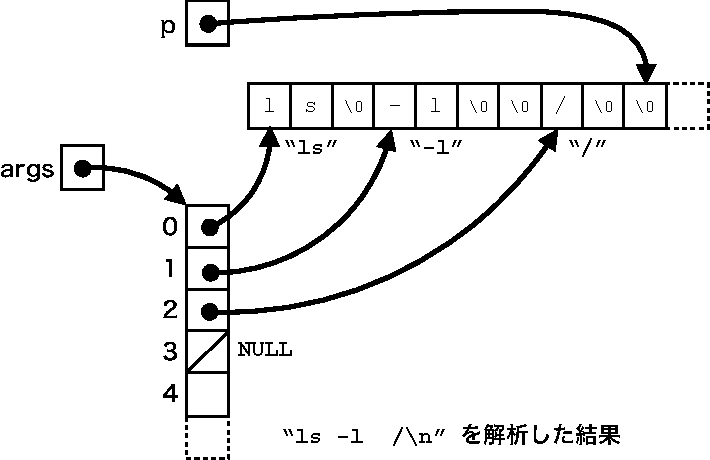
\includegraphics[scale=0.8]{Fig/myshellArgs-crop.pdf}
\end{myfig}

\figref{myshellArgs}に\|parse()|関数実行後のデータ構造の例を示す.
この例は,コマンド行文字列
~\texttt{"ls{\textvisiblespace}-l{\textvisiblespace}{\textvisiblespace}/{\bs}n"}~
を解析した後のデータ構造である.
渡された文字列の空白を\|'\0'|で上書きし
\|"ls"|,\|"-l"|,\|"/"|の3つの文字列が作られている\footnote{
  リスト\ref{myshellParse}の5行で\texttt{'{\bs}0'}に書換えている.}.
文字列配列の終端は\|NULL|で表現する.
\|args|配列は各文字列の先頭を指すポインタを格納する\footnote{
  リスト\ref{myshellParse}の7行でポインタを\texttt{args}配列に格納している.
}ことで文字列配列を表現する.
文字列の最後の \|'\n'| は \|'\0'| に書き換わっている\footnote{
  \texttt{'{\bs}n'}は\texttt{isspace()}関数により空白と判断される.
}.

\subsection{コマンドの実行(\texttt{execute()})}
リスト\ref{myshellExecute}にmyshellの\|execute()|関数を示す.
この関数は\|parse()|関数が作った\|args|配列を受け取り,
内部コマンドなら自分で実行し,
外部コマンドなら子プロセスを作って実行させる.

\lstinputlisting[label=myshellExecute
  ,caption=コマンドの実行ルーチン(\texttt{execute()})
  ,float=btp, numbers=left, firstline=22, lastline=44]{Lst/myshell.c}

2行ではコマンドの名前を調べている.
cd コマンドは内部コマンドなので,
5行で自ら\|chdir()|システムコールを実行している\footnote{
  内部コマンドを追加するときは,cd コマンドと同様に,ここに追加する.}.
7行以下は外部コマンドの処理である.
9行で子プロセスを作り,14行で子プロセスがコマンドを実行する.
親プロセスは18行で子プロセスの終了を待つ.

14行では\|execve()|システムコールの代わりに\|execvp()|関数を用いているので,
PATH環境変数を用いたプログラムの自動的な探索が行われる.

%=============================================================================
\newpage
\section*{課題 No.11}

\begin{enumerate}
\item myshell に環境変数を追加するコマンド setenv ,
  削除するコマンド unsetenv を追加しなさい.
\item myshell にリダイレクト機能を追加しなさい.
\end{enumerate}

\subsection*{機能追加後のmyshellの実行例(参考)}
\begin{lstlisting}[numbers=none]
Command: setenv A B
Command: printenv A
B
Command: unsetenv A
Command: printenv A
Command: echo aaa > a.txt
Command: cat a.txt
aaa
Command:
\end{lstlisting}
 % myShell

%------------------------------------------------------------------------------
% 発行元
\backmatter
\pagestyle{empty}
\onecolumn
~
\vfill\vfill\vfill
\begin{center}
\fbox{\parbox{10cm}{ \vspace{0.3cm}
\large{\textbf{システムプログラミング Ver. 0.0.0}} \\
\\
 発行年月 2018年06月 Ver.0.0.0 \\
 発  行 独立行政法人国立高等専門学校機構 \\
      徳山工業高等専門学校 \\
      情報電子工学科 重村哲至 \\
      〒745-8585 山口県周南市学園台 \\
      sigemura@tokuyama.ac.jp \\
}}
\end{center}
\vfill
\end{document}
